


\documentclass[10pt]{beamer}
%
% Choose how your presentation looks.
%
% For more themes, color themes and font themes, see:
% http://deic.uab.es/~iblanes/beamer_gallery/index_by_theme.html
%
\mode<presentation>
{
  \usetheme{CambridgeUS}      % or try Darmstadt, Madrid, Warsaw, ...
  \usecolortheme{dolphin} % or try albatross, beaver, crane, ...
  \usefonttheme{default}    % or try serif, structurebold, ...
  \setbeamertemplate{navigation symbols}{}
  \setbeamertemplate{caption}[numbered]

}


\usepackage[spanish]{babel}
\usepackage{hyperref}
\usepackage[utf8x]{inputenc}
\usepackage{epstopdf}
\usepackage[caption = false]{subfig}
%\usepackage[dvipsnames]{xcolor}
\usepackage{color, colortbl}
\definecolor{Gray}{gray}{0.9}
\usepackage{amssymb} 
\usepackage{amsmath}
\usepackage{multicol}


%\setbeamersize{text margin left=0.1cm,text margin right=0.1cm}




%\setbeamercolor{block title}{bg=red!30,fg=black}  %Definir el color de las cajas




%-=-=-=-=-=-=-=-=-=-=-=-=-=-=-=-=-=-=-=-=-=-=-=-=
%S
%	TITLE PAGE
%
%-=-=-=-=-=-=-=-=-=-=-=-=-=-=-=-=-=-=-=-=-=-=-=-=


%Between brackets is the shorter name ()
\title[ATLAS Open Data 13 TeV: Física del Top]{Primer análisis de física del quark top 
\\
utilizando el ATLAS OPEN DATA a \\$\sqrt{s}=13$ TeV y $L_{\text{int}}=3.2$ fb$^{-1}$ (2015)} 
\subtitle{IFIC's Severo Ochoa Summer Student School: 9-20 July 2018}
\author[Á. Ruiz García y C. Falcó i Gandia]{Álvaro Ruiz García y Carlos Falcó i Gandia}
\institute[ UV and UAB ]{UV and UAB} 


% 		For mulptiple authors
\author[Á. Ruiz García y C. Falcó i Gandía]{Álvaro Ruiz García  \inst{1} \\ Carles Falcó i Gandia\inst{2}\\}
\institute
{
 \inst{1}%
  Universidad de Valencia
  \and
  \inst{2}%
  Universidad Autónoma de Barcelona
  \and Tutor: Susana Cabrera, en coordinación con el grupo ATLAS-OUTREACH (Meirin Oan Evans y Arturos Sánchez Pineda)
}
\date{\today}


%\titlegraphic{\includegraphics[width=2cm]{/afs/ific.uv.es/user/p/pamarag/public/plots/LaTeX/t-channel:14-09/Figures/IFIC-Logo.jpg}\hspace*{4.75cm}~%
%   \includegraphics[width=3cm]{/afs/ific.uv.es/user/p/pamarag/public/plots/LaTeX/t-channel:14-09/Figures/ATLAS-Logo-Ref-CMYK-H_0.jpg}
%}



%\definecolor{MyBackground}{RGB}{255,241,167}
%\setbeamercolor{background canvas}{bg=MyBackground}


\begin{document}

\begin{frame}
  \titlepage
\end{frame}





%-=-=-=-=-=-=-=-=-=-=-=-=-=-=-=-=-=-=-=-=-=-=-=-=
%
%	TABLE OF CONTENTS: OVERVIEW
%
%-=-=-=-=-=-=-=-=-=-=-=-=-=-=-=-=-=-=-=-=-=-=-=-=
% Uncomment these lines for an automatically generated outline.
\begin{frame}{Contenido}
  \tableofcontents

\end{frame}


\section{Estudio de la producción de un sólo top (single-top) en el canal t}


\subsection{Estudio a nivel de generador}

\begin{frame}{Estudio a nivel de generador}
 $$t\longrightarrow Wb\longrightarrow l\nu b$$
	\begin{figure}
	\centering
	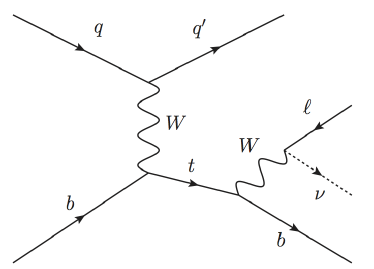
\includegraphics[scale=0.345]{tchannel.png}
	\caption{Diagrama de Feynman proceso $t$-channel}
\end{figure}

$$p^W = p^l + p^\nu\quad\qquad p^t = p^W+p^b = p^l + p^\nu +p^b$$

\end{frame}
\begin{frame}
\begin{center}
\begin{tabular}{ccc}

	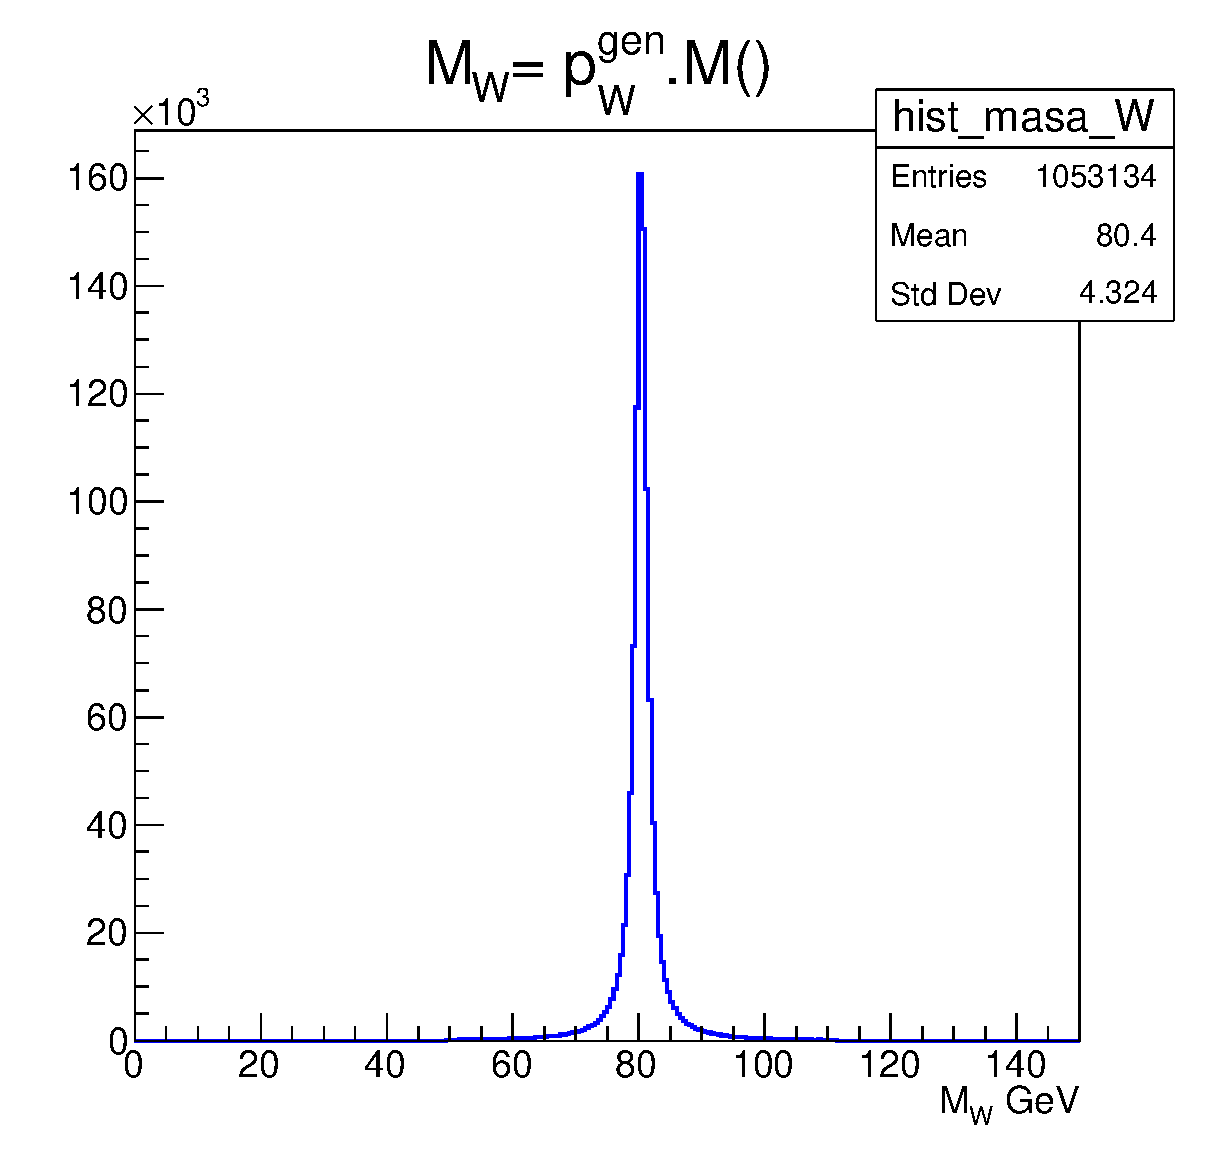
\includegraphics[scale=0.18]{plot-gen-mw.eps} &&

	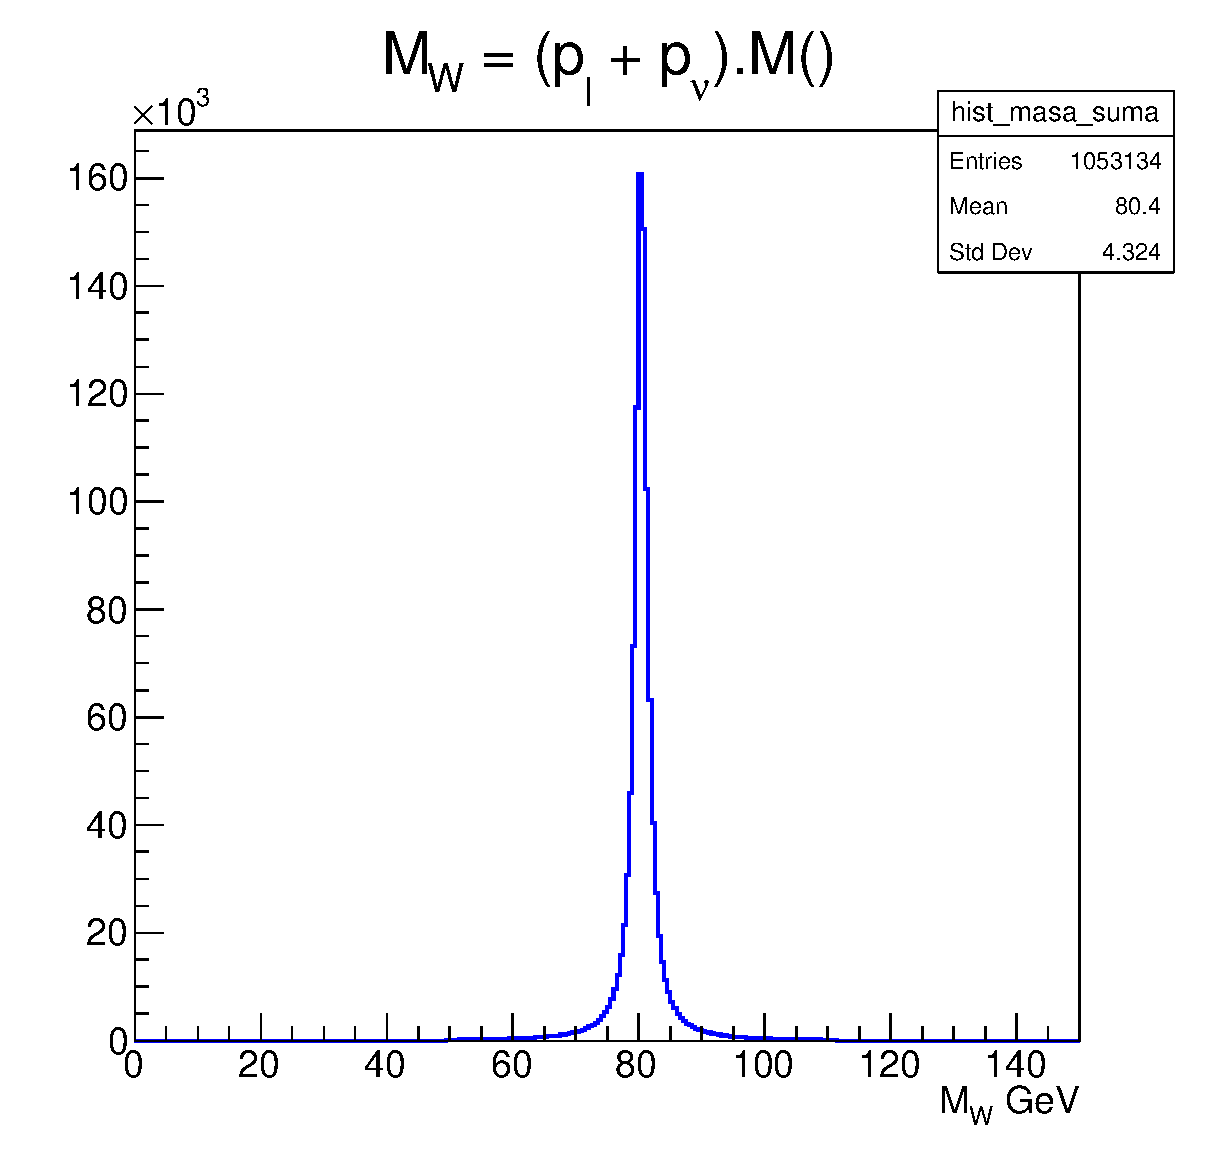
\includegraphics[scale=0.18]{plot-mw-reco.eps} \\

	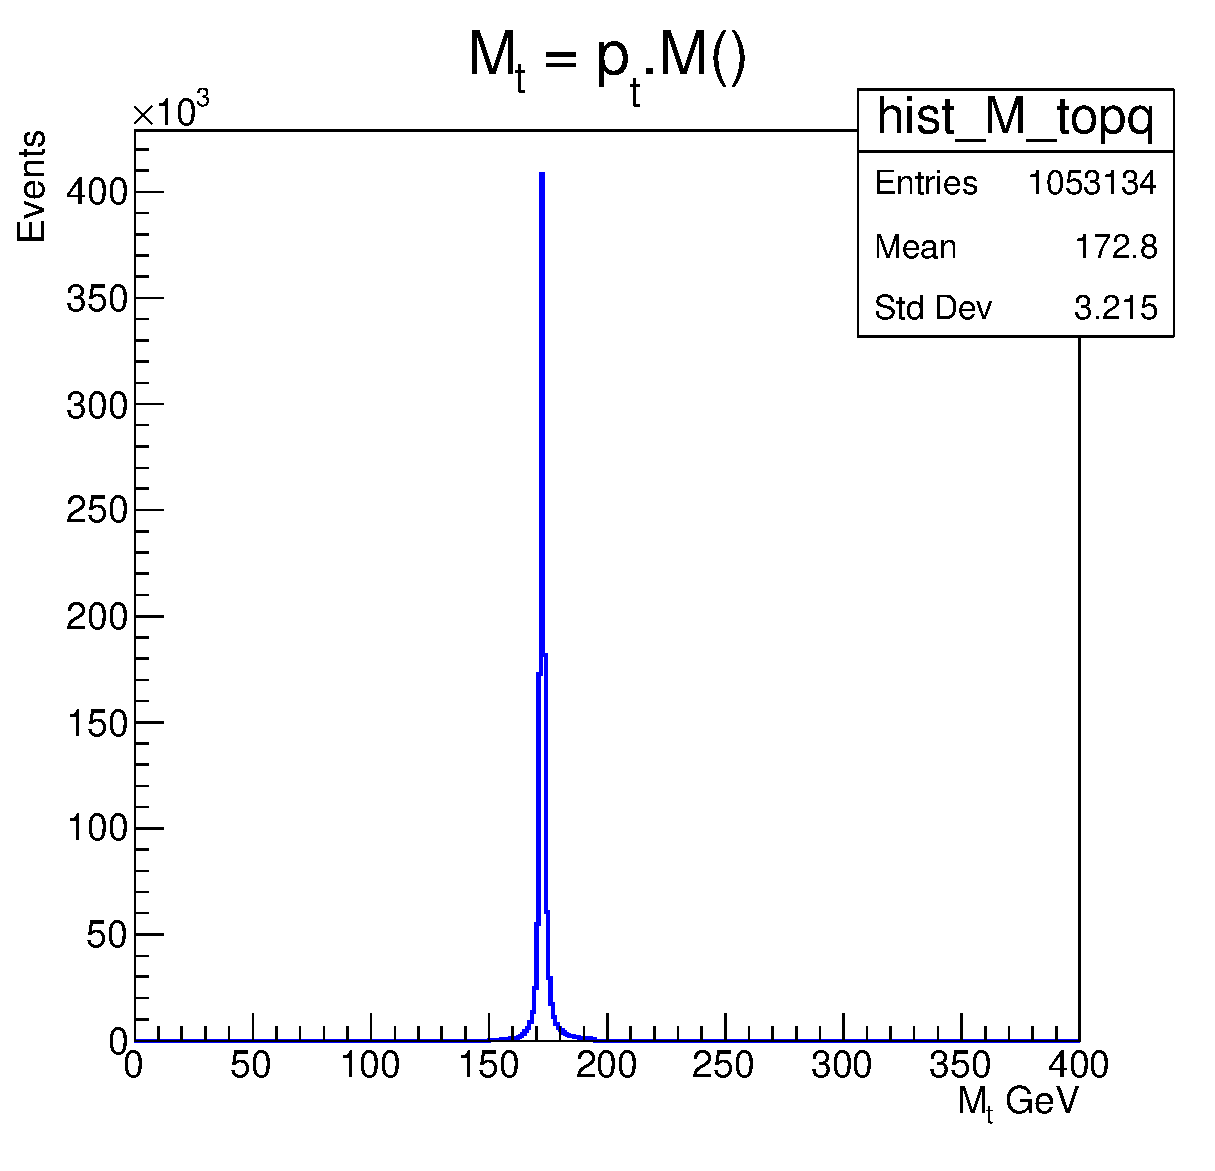
\includegraphics[scale=0.18]{plot-mtop-gen.eps} &

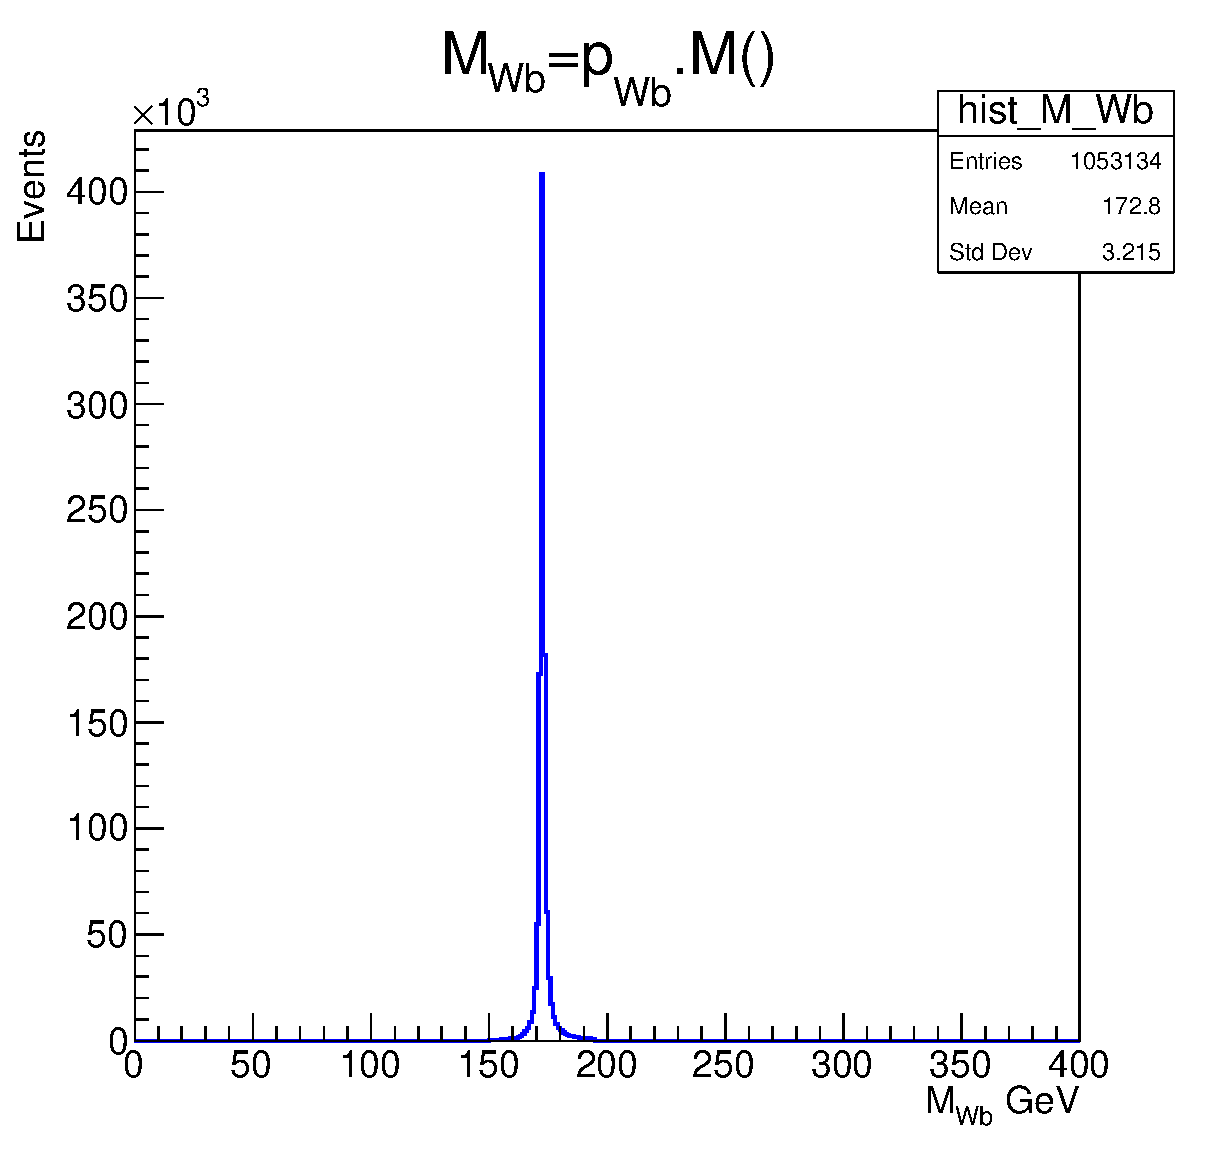
\includegraphics[scale=0.18]{plot-mWb-gen.eps}&
	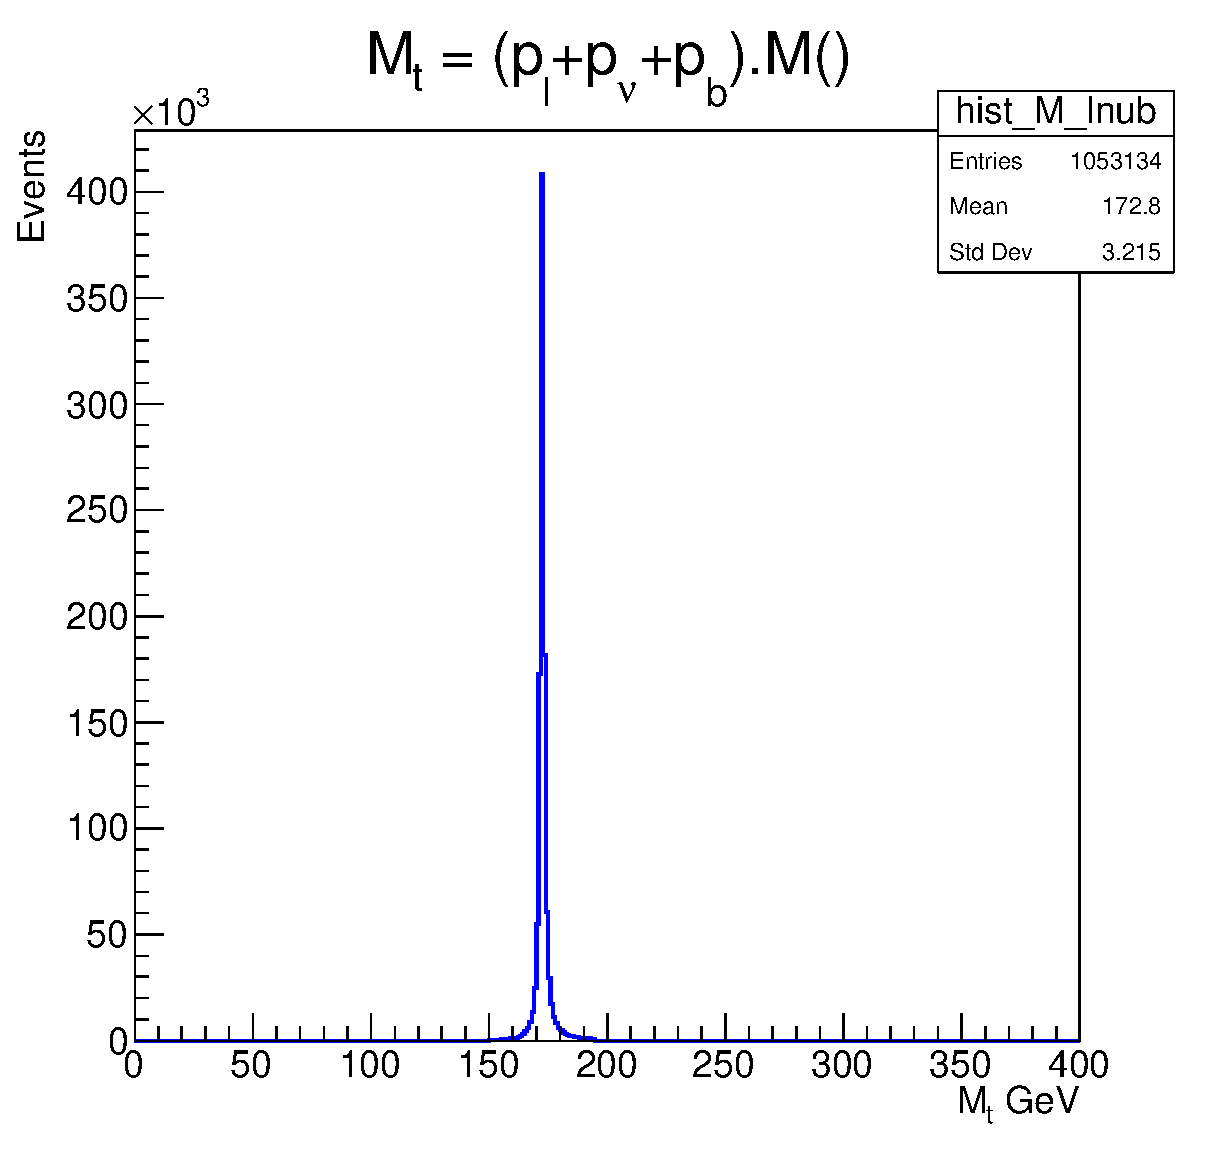
\includegraphics[scale=0.18]{plot-mtop-reco.eps} 
	
	

\end{tabular}
\end{center}
\end{frame}

\subsection{Estudio de reconstrucción de la masa}

\begin{frame}{Estudio de reconstrucción de la masa.}

\color{blue}{Determinación del momento longitudinal del neutrino}

 \color{olive}{The ATLAS collaboration, Aaboud, M., Aad, G. et al. J. High Energ. Phys. (2017) 2017: 17}
\color{black}
\begin{equation*}
	(p^W)^2=(p^l +p^{\nu})^2
\end{equation*}
\begin{equation*}
	(E_T^{\text{miss}})^2=(p_T^{\nu})^2+(p_z^{\nu})^2 \qquad\quad E^{\nu}=\sqrt{(E_T^{\text{miss}})^2+(p_z^{\nu})^2}
\end{equation*}
\begin{equation*}
	a(p_z^{\nu})^2+b p_z^{\nu}+c=0\longrightarrow
	\begin{cases}
	 a=(E^l)^2-(p^l_z)^2 \\
	 b=p_z^l\big(-m_W^2+m_l^2-2(p_x^lp_x^{\nu}+p_y^lp_y^{\nu}) \big) \\
	c= (E^l)^2(E_T^{\text{miss}})^2-\frac{1}{4}\big(m_W^2-m_l^2+2(p_x^lp_x^{\nu}+p_y^lp_y^{\nu})\big)^2
	\end{cases}
\end{equation*}
\begin{equation*}
	\Delta=(E_l)^2\Big[\big(m_W^2-m_l^2+2(p_x^lp_x^{\nu}+p_y^lp_y^{\nu})\big)^2+4(E_T^{\text{miss}})^2\big(-(E^l)^2+(p_z^l)^2\big)\Big]
\end{equation*}

\begin{itemize}
	\item $\Delta >0\; (\approx70\%) \longrightarrow $ Solución con menor $p_z$
	\item $\Delta <0\; (\approx30\%)\longrightarrow\begin{cases}
	\circ \quad \Delta =0 \\ \circ \quad \text{Se calcula } E_T^{\text{miss}} \text{ tal que } \Delta =0 \text{. }\\ E_T^{\text{miss}}={E_T^{\text{miss}}}'+\delta \text{ tal que } \Delta >0
	\end{cases}$ 
\end{itemize}
\end{frame}

\begin{frame}
	\begin{center}
		\begin{tabular}{ccc}
			
			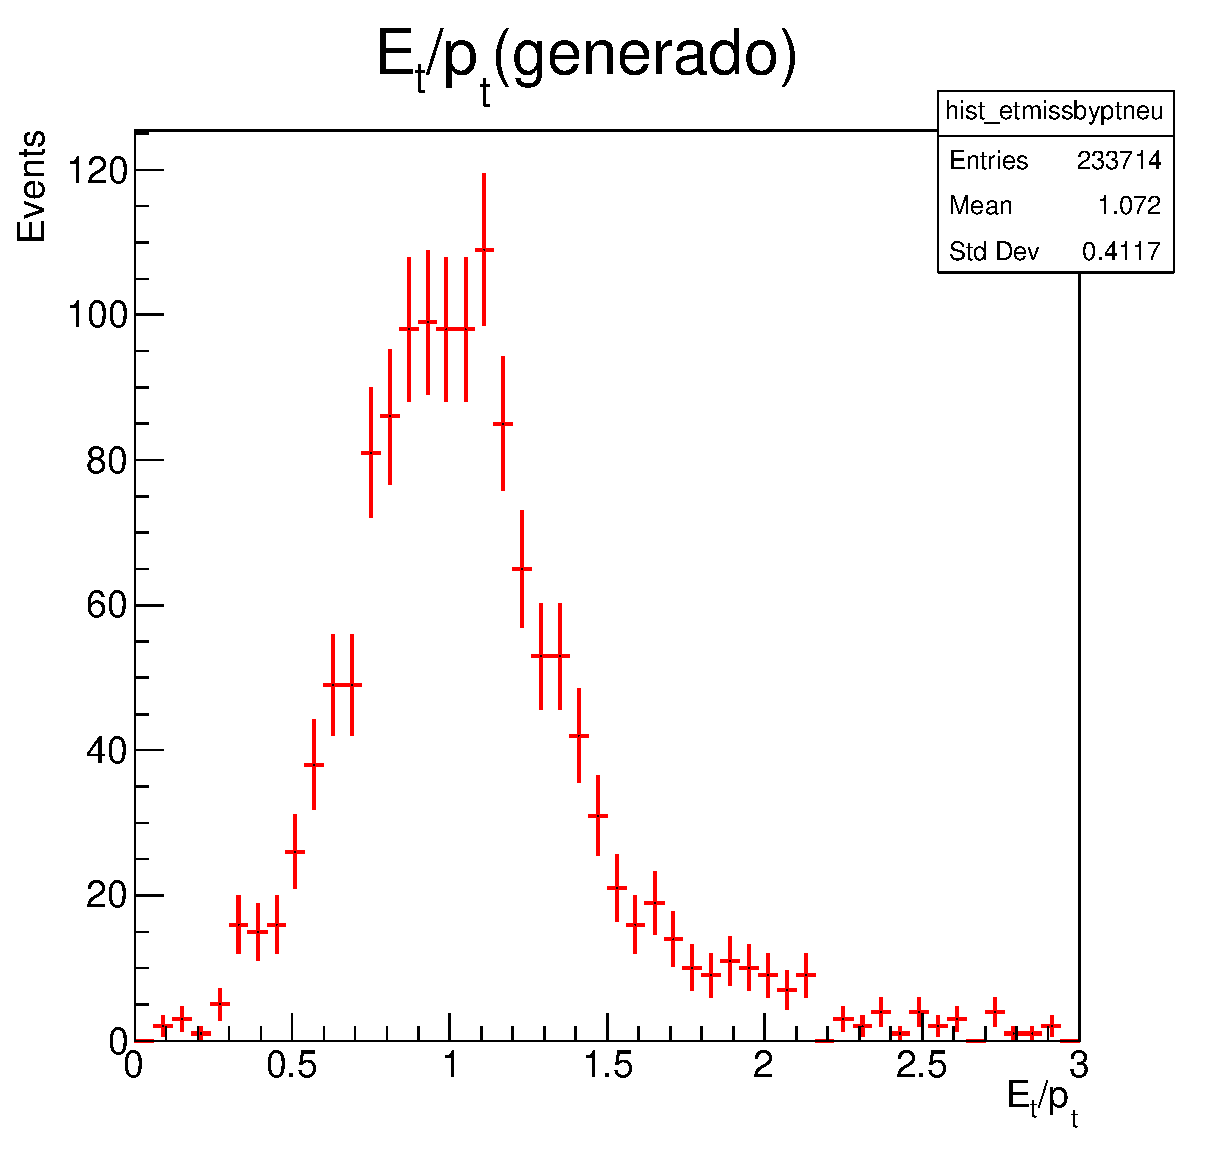
\includegraphics[scale=0.18]{plot-etmissbyptneu.eps} &
				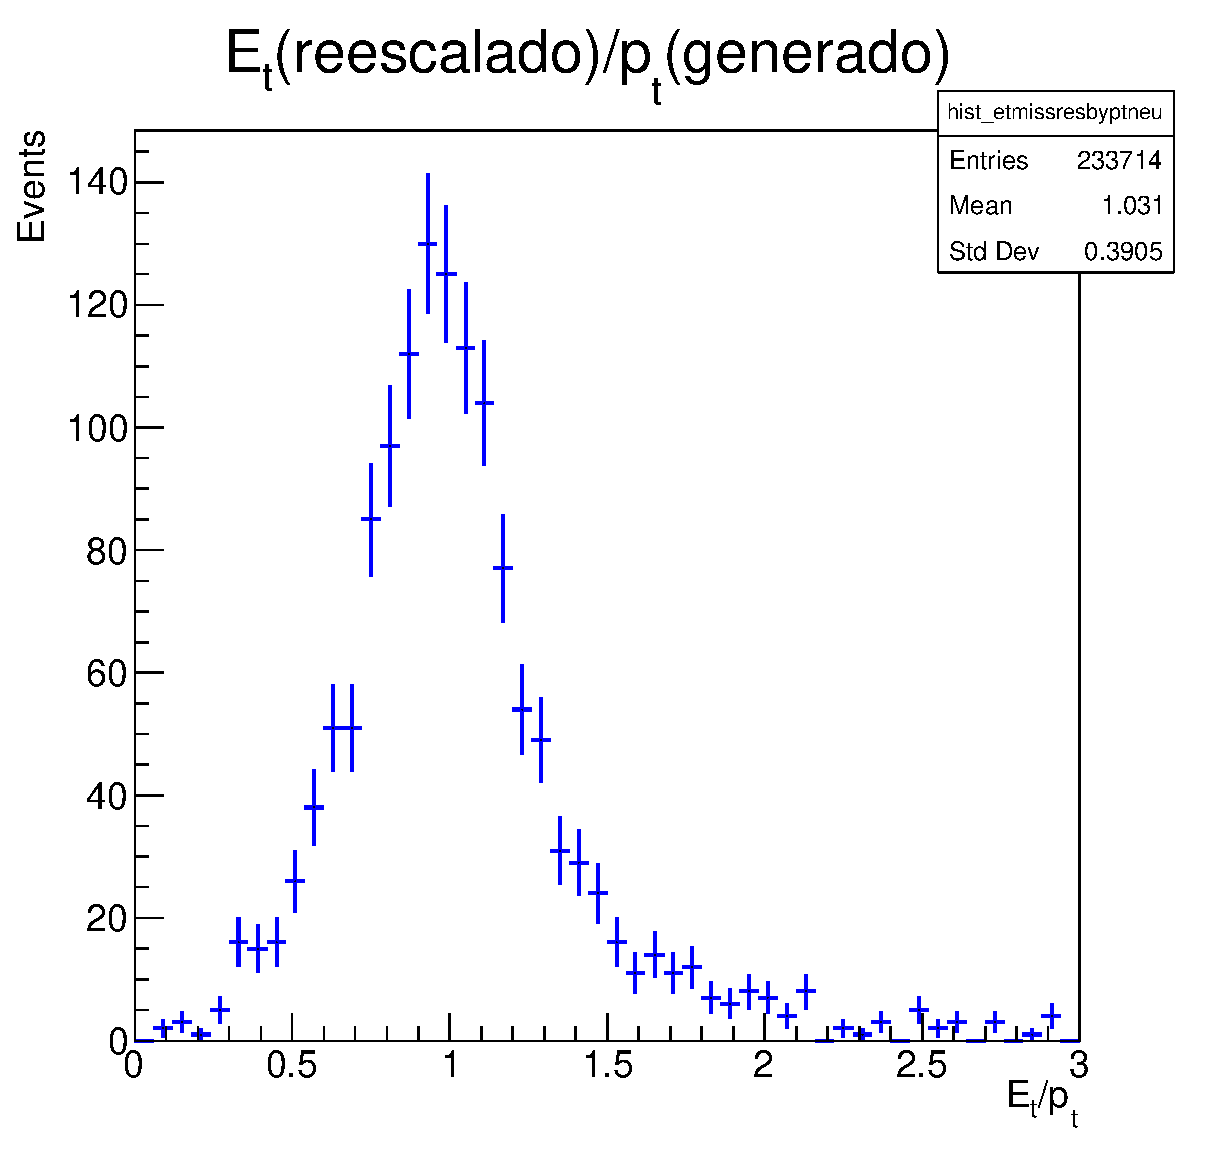
\includegraphics[scale=0.18]{plot-etmissresbyptneu.eps}&
				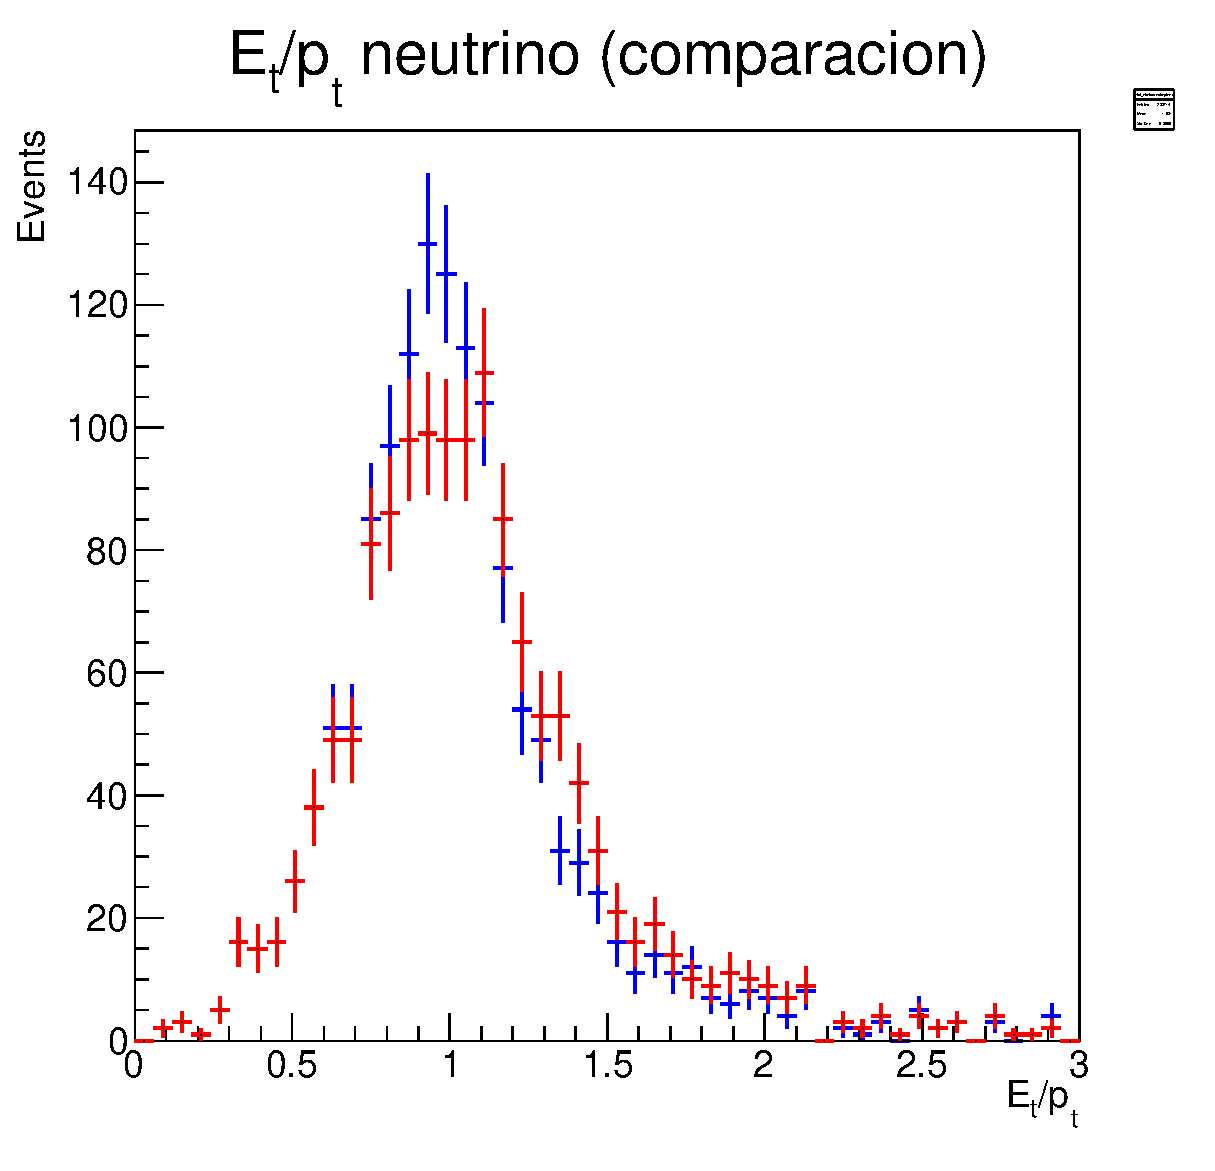
\includegraphics[scale=0.18]{plot-etmisscomparation.eps}
				
			
		 \\
			
			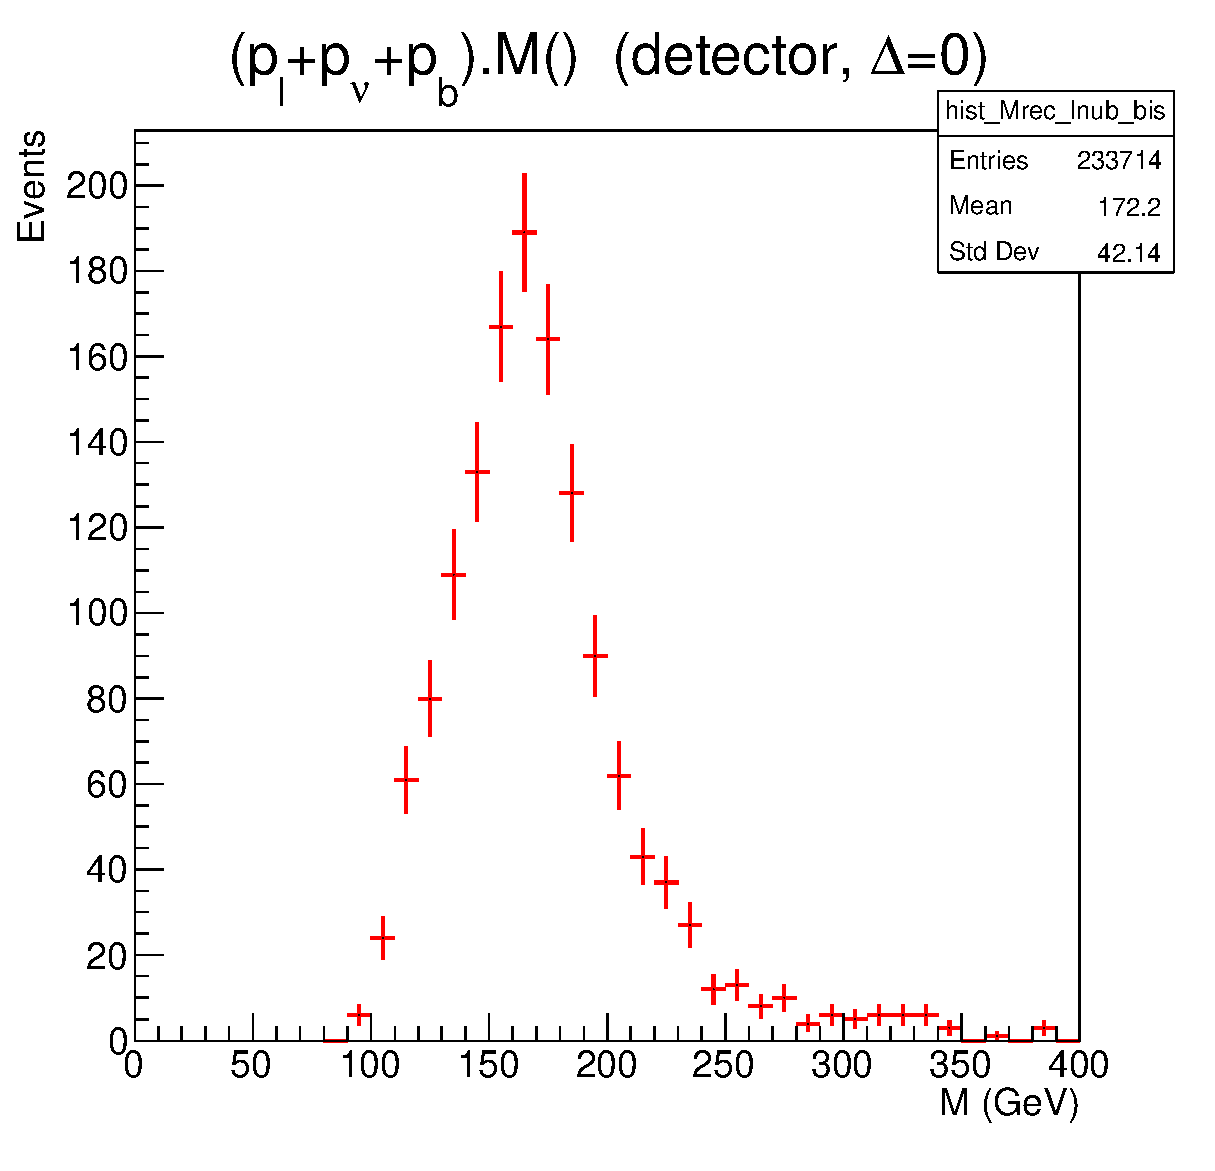
\includegraphics[scale=0.18]{plot-mt-reco-det-bis.eps} &

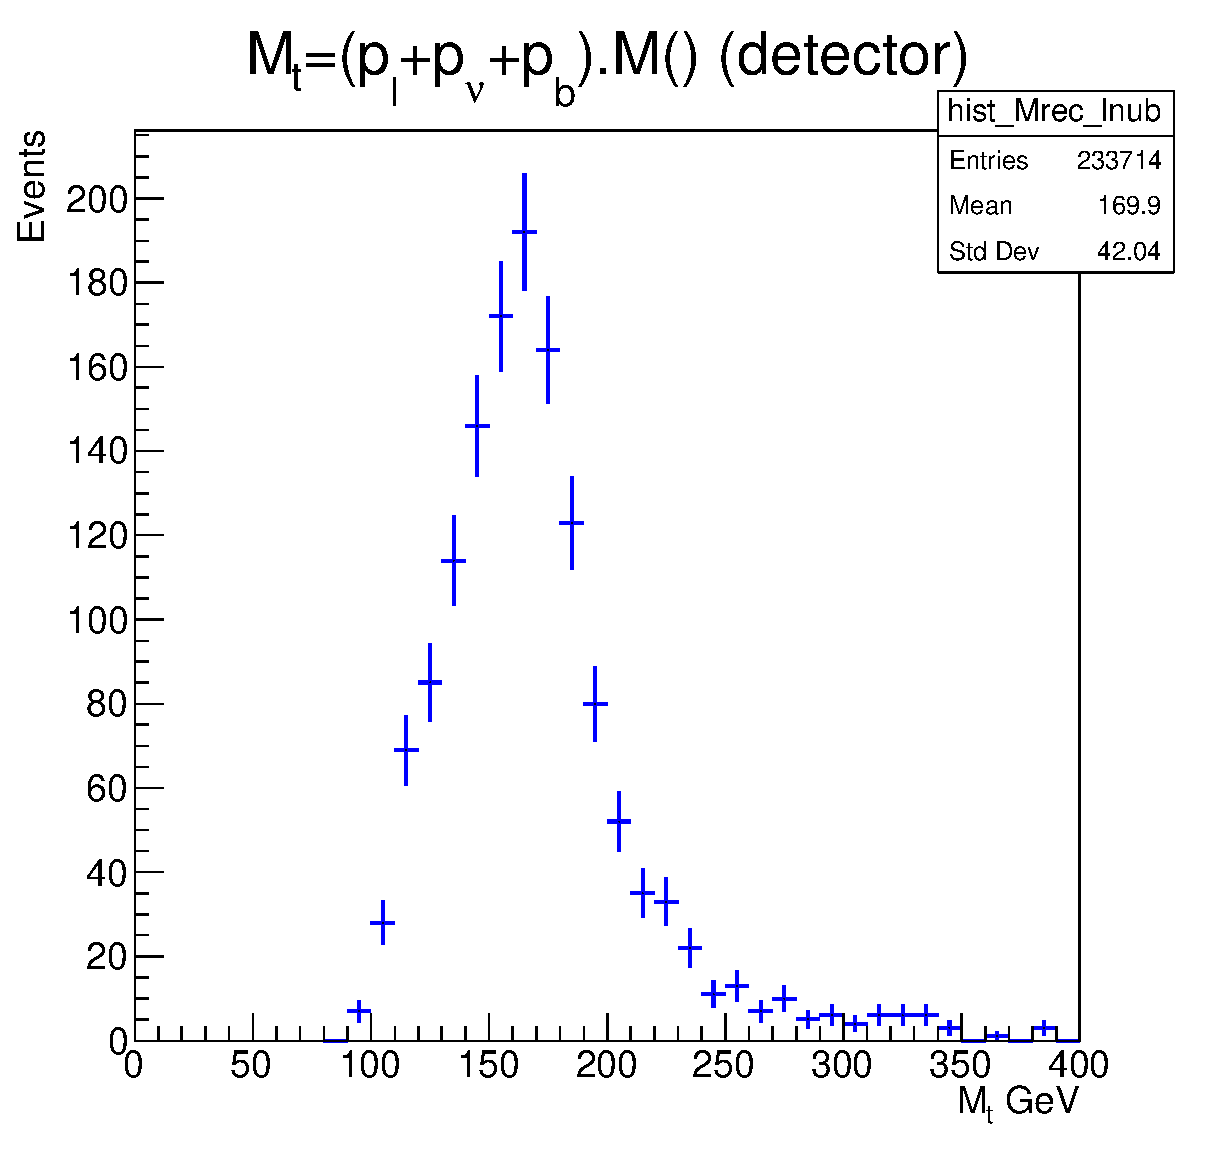
\includegraphics[scale=0.18]{plot-mt-reco-det.eps} &
			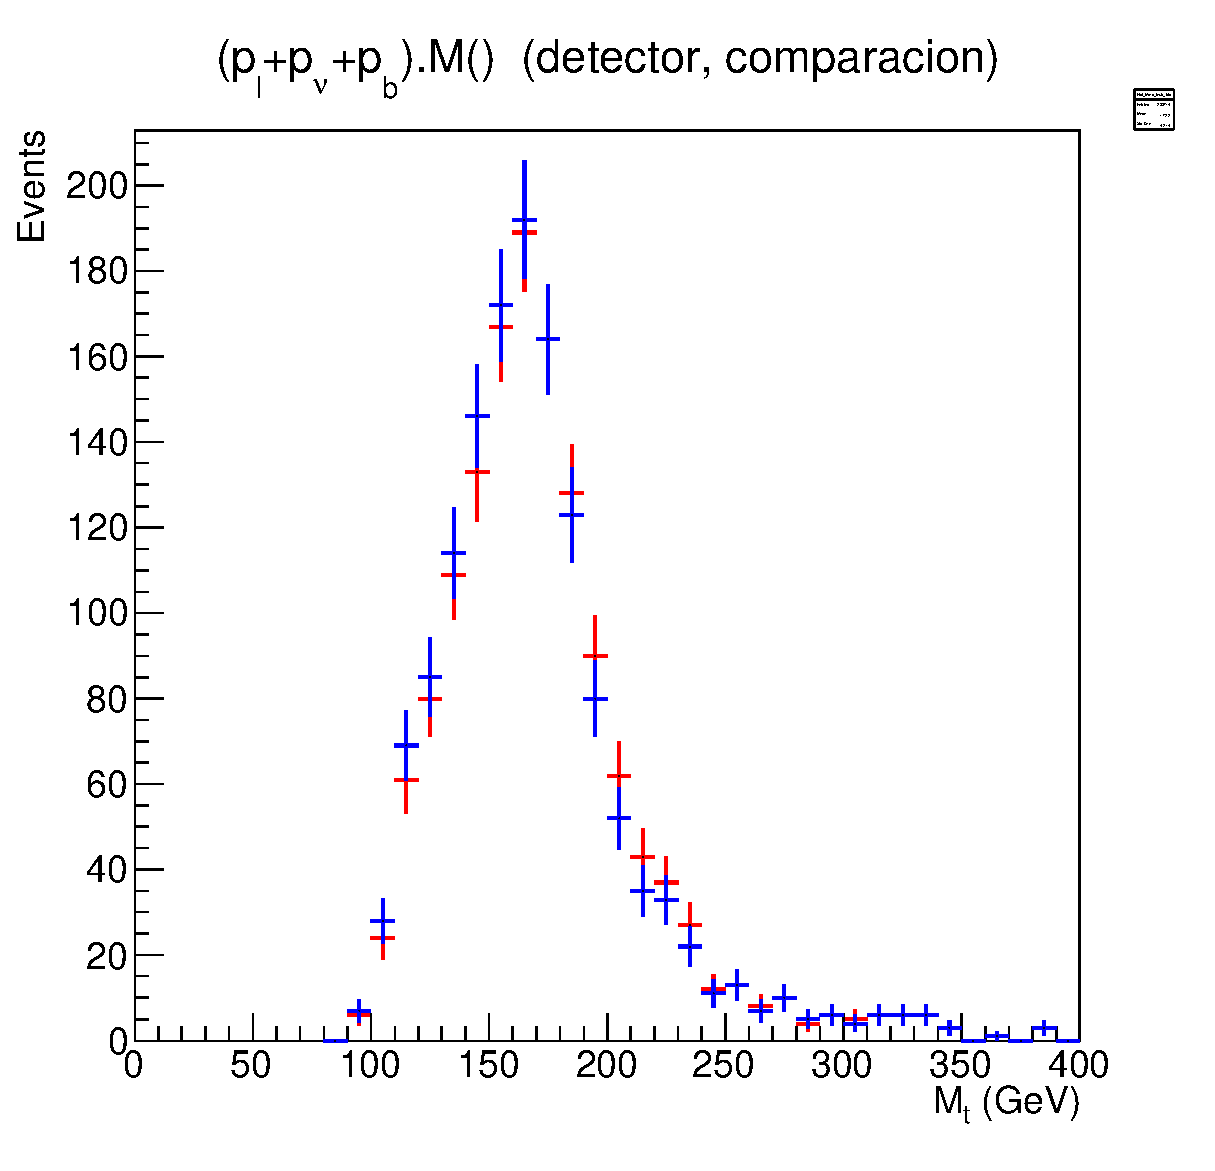
\includegraphics[scale=0.18]{plot-mt-reco-det-comparacions.eps} 
			
			
			
		\end{tabular}
	\end{center}
\end{frame}
\subsection{Estudio de selección de señal single-top canal t y rechazo de fondos.}

\begin{frame}{Estudio de selección de señal single-top canal t y rechazo de fondos}
\begin{columns}
	\begin{column}{.65\textwidth}
		\color{blue}	Cortes previos (preselección):
	\begin{itemize}
		\item Trigger de leptones y criterios de calidad del evento
		\item 1 leptón cargado ($e$ o $\mu$) y aislado
		\item $E_T^{\text{miss}}>30 $ GeV y $M_T^{W}>50$ GeV  (reducir QCD)
		\item 2 jets y 1 b-jet (mv2c10$>$0.7892)
	\end{itemize}
\end{column}
	\begin{column}{.3\textwidth}
		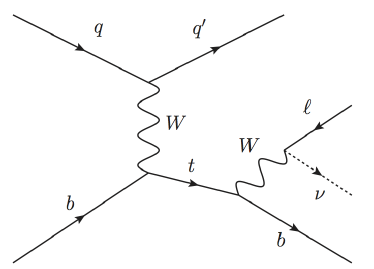
\includegraphics[scale=0.25]{tchannel.png}
	\end{column}
\end{columns}
\begin{columns}
	\begin{column}{.65\textwidth}
		\color{blue}	Cortes de selección:
			
		\color{olive}{The ATLAS collaboration, Aaboud, M., Aad, G. et al. J. High Energ. Phys. (2017) 2017: 124}
		\begin{itemize}
			\item Pseudorapidity del light jet $|\eta|>1.5$
			\item $|\eta_l-\eta_b|>1.5$
			\item $H_t=p_t^l+ p_t^{\text{light jet}}+p_t^{\text{b-jet}} + E_T^{\text{miss}} >195$ GeV
			\item $150$ GeV $<M_{\text{top}}<$ 220 GeV
		\end{itemize}
	\end{column}
	\begin{column}{.3\textwidth}
		$$\eta = -\ln\big[\tan\big(\tfrac{\theta}{2}\big)\big]
$$		
\includegraphics[scale=0.33]{eta.png}
	\end{column}
\end{columns}
% PLOTS.. mtop, variables utilizadas en los cortes antes d elos mismos:
% i.e, después de requerir: 1 leptón, 2jets, 1bjet, etmiss>30, mtw>50
% TABLA S,B,S/B,S/sqrt(S+F) cortes secuenciales (Carlos)
% TABLA S,B,S/B,S/sqrt(S+F) antes y después de todos los cortes (Álvaro)
\end{frame}
\begin{frame}
	\begin{center}
		\begin{tabular}{cc}
			
			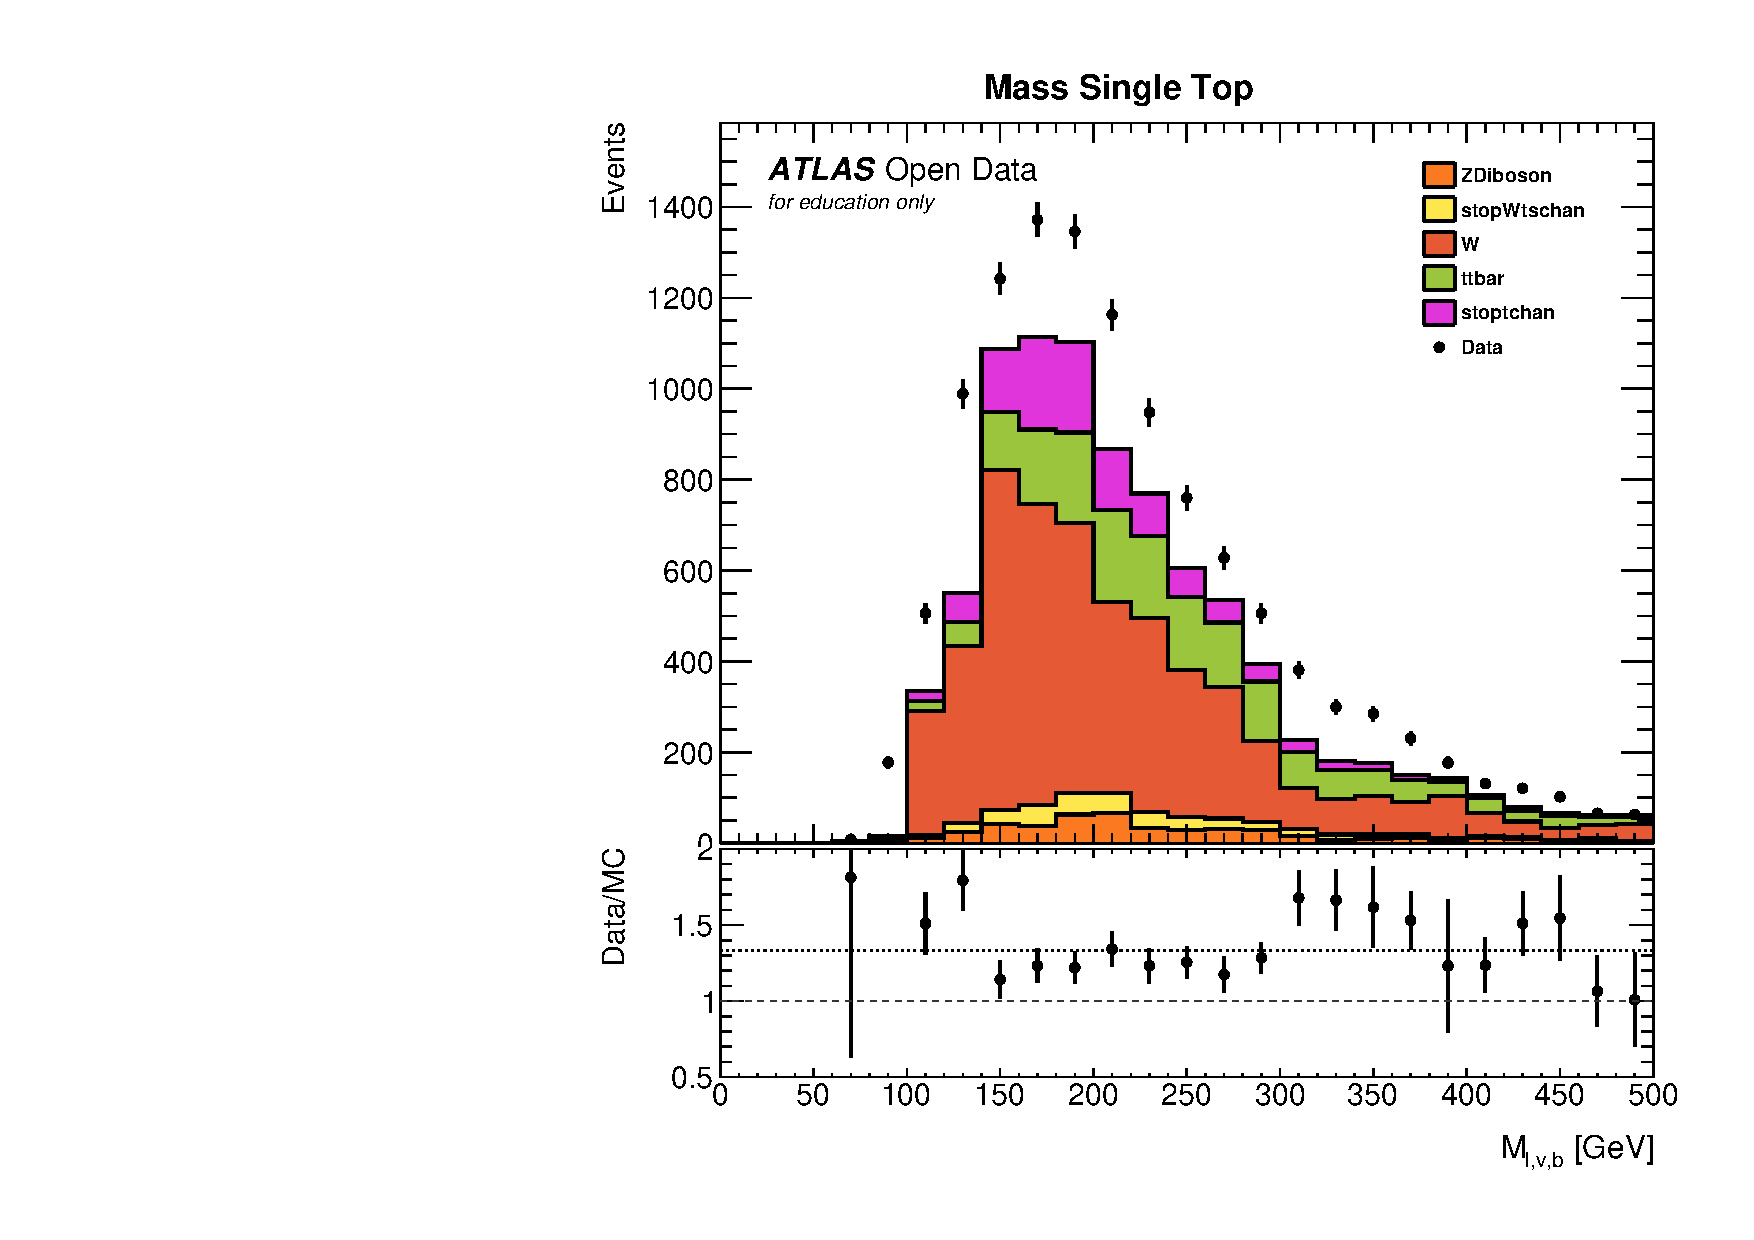
\includegraphics[scale=0.22]{SingleTopMass} &
			
			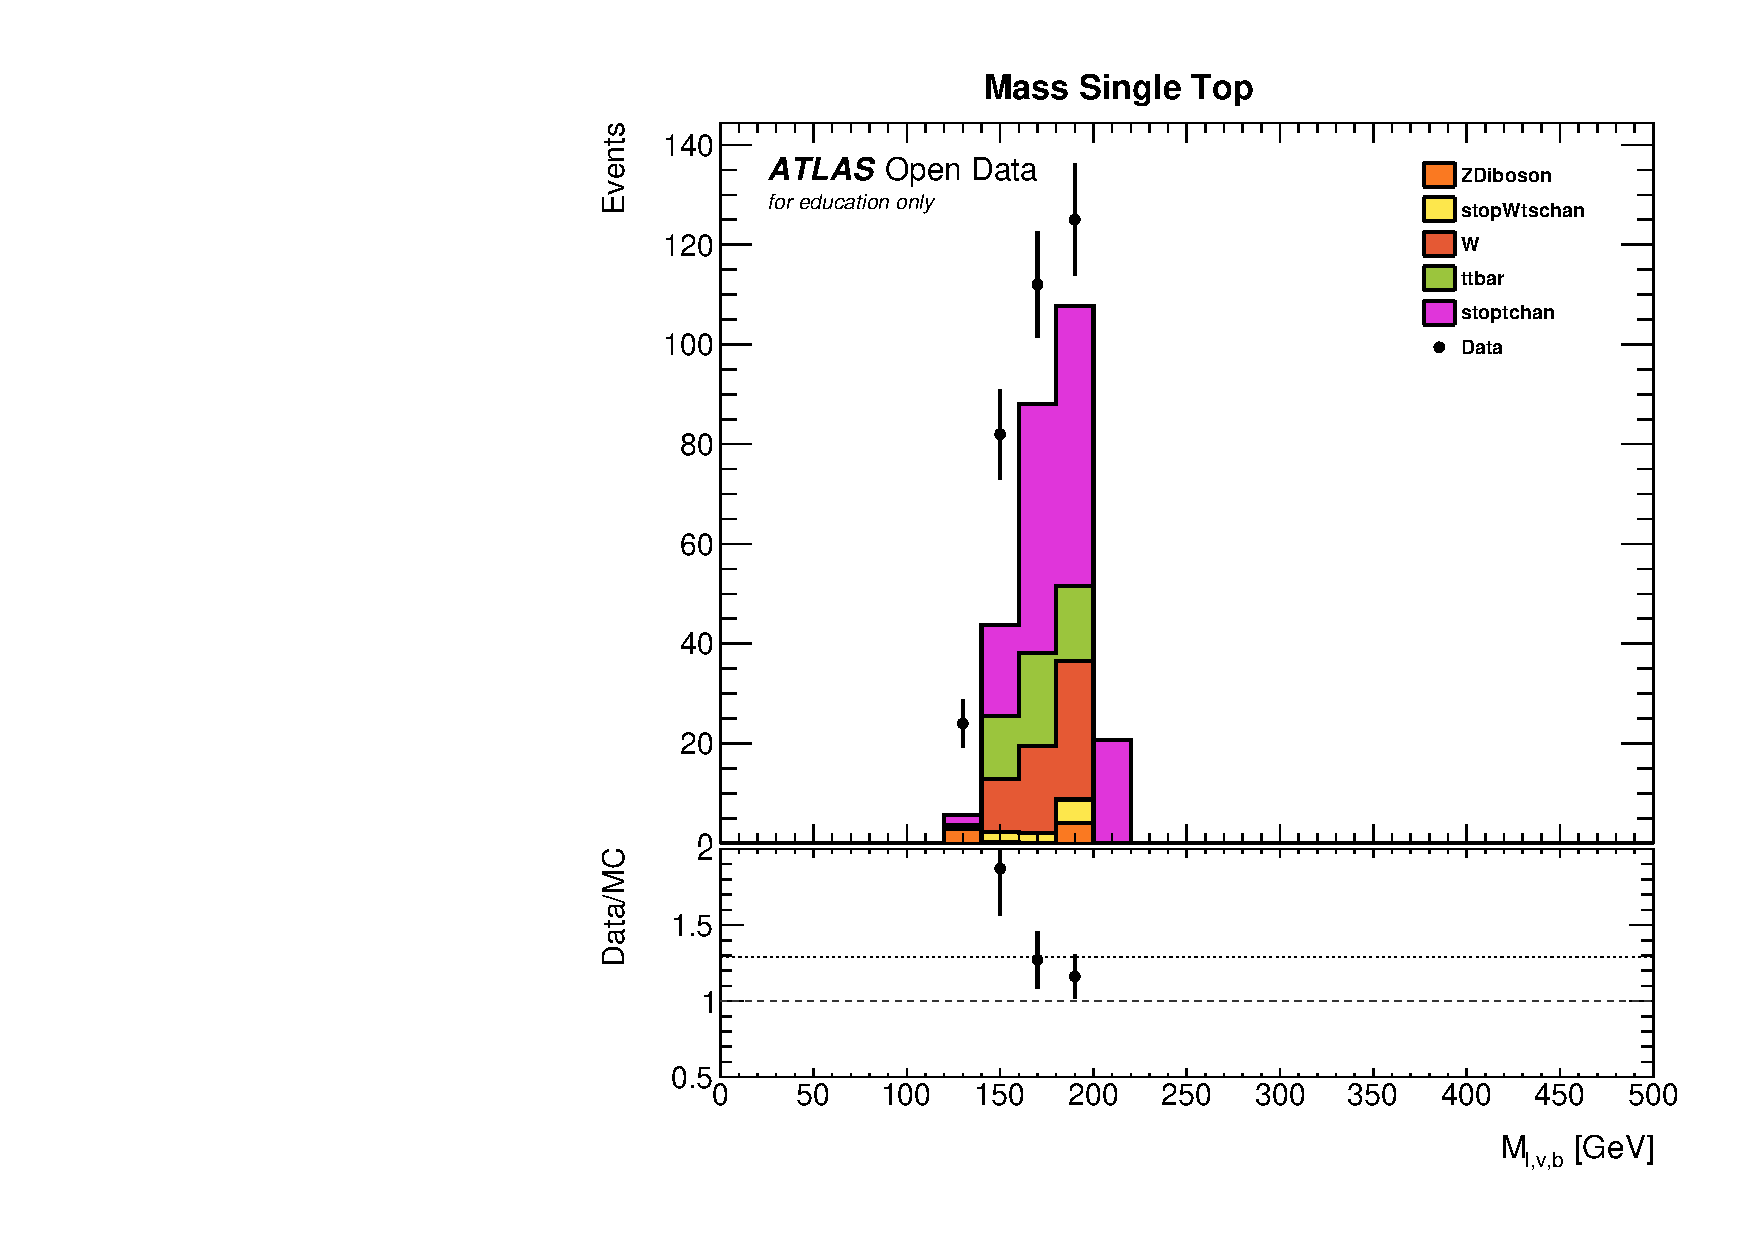
\includegraphics[scale=0.22]{SingleTopMass_cuts} \\
			
			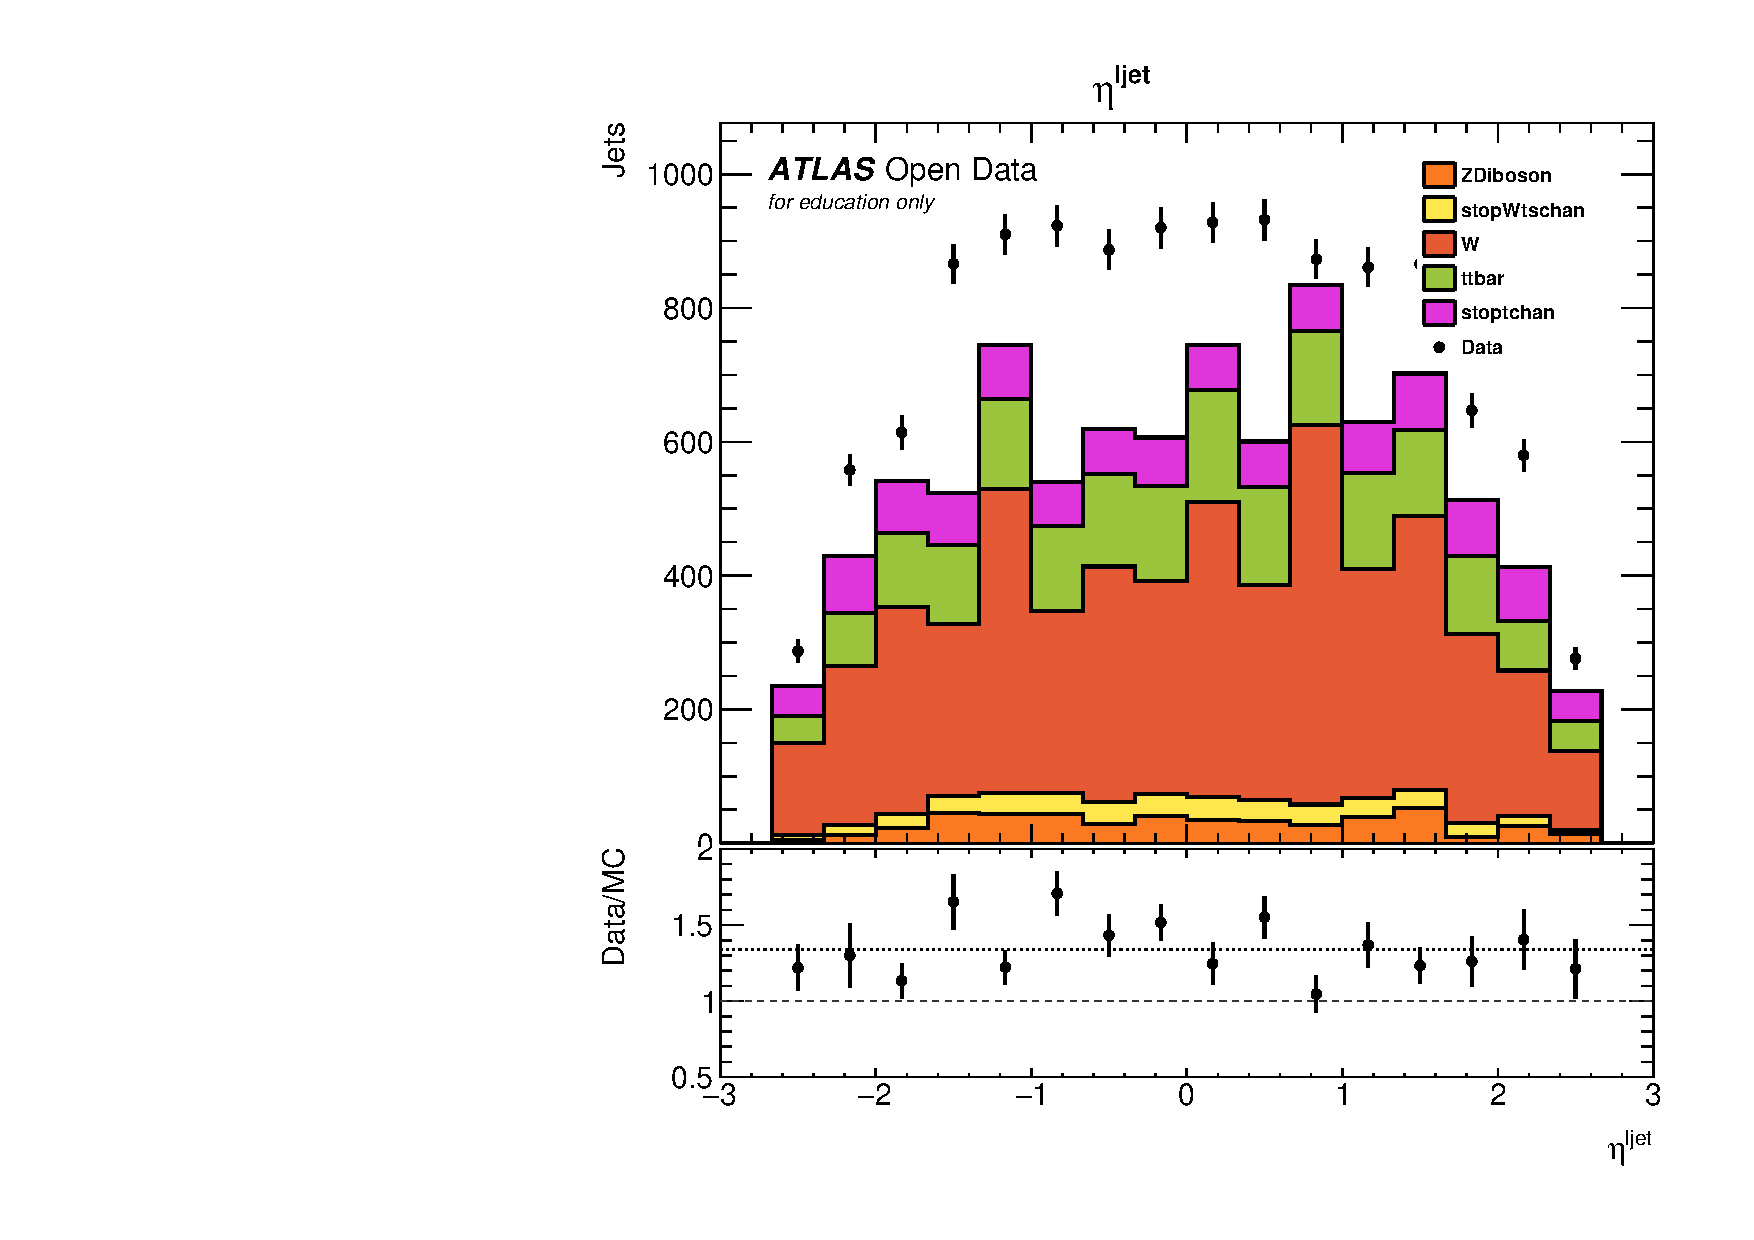
\includegraphics[scale=0.22]{qEta} &
			
		
			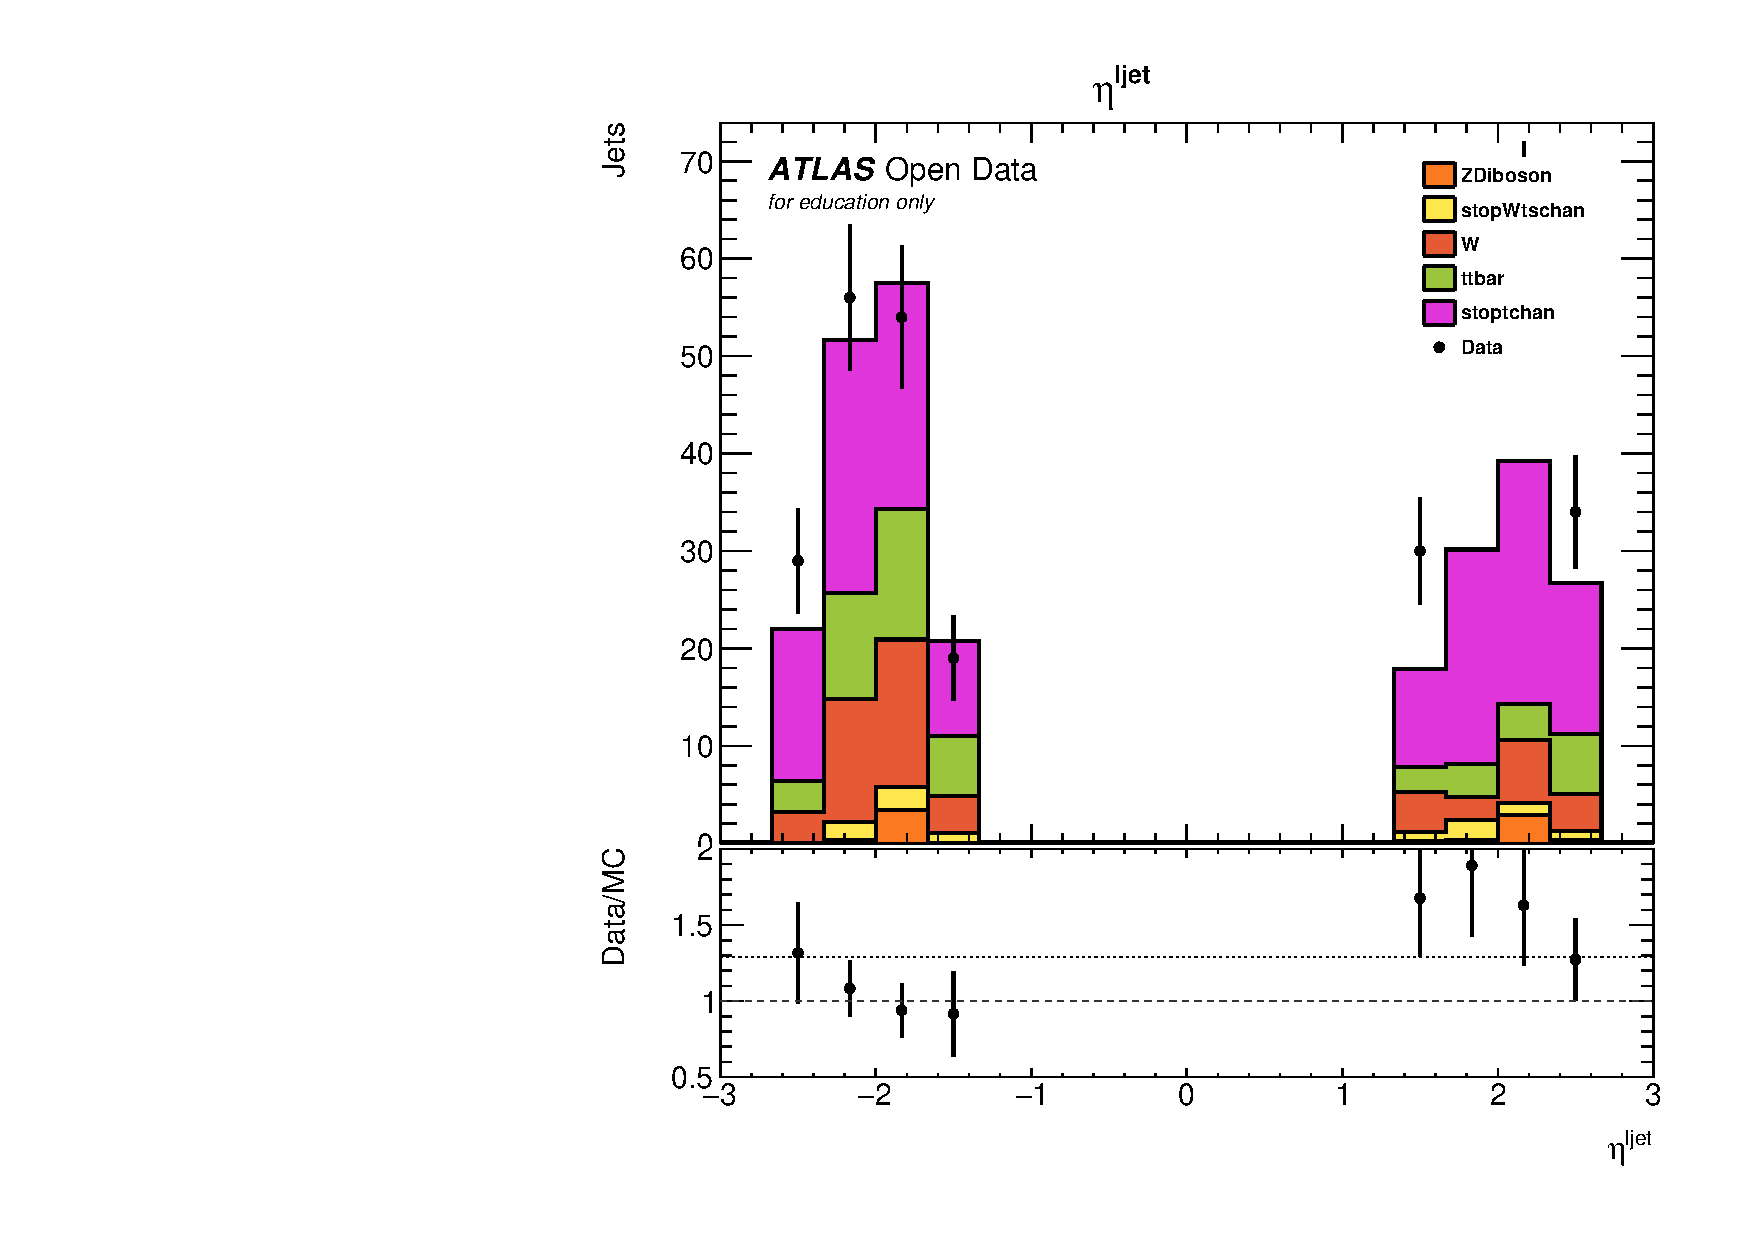
\includegraphics[scale=0.22]{qEta_cuts} 
			
			
			
		\end{tabular}
	\end{center}
\end{frame}
\begin{frame}
\begin{center}
	\begin{tabular}{cc}
		
		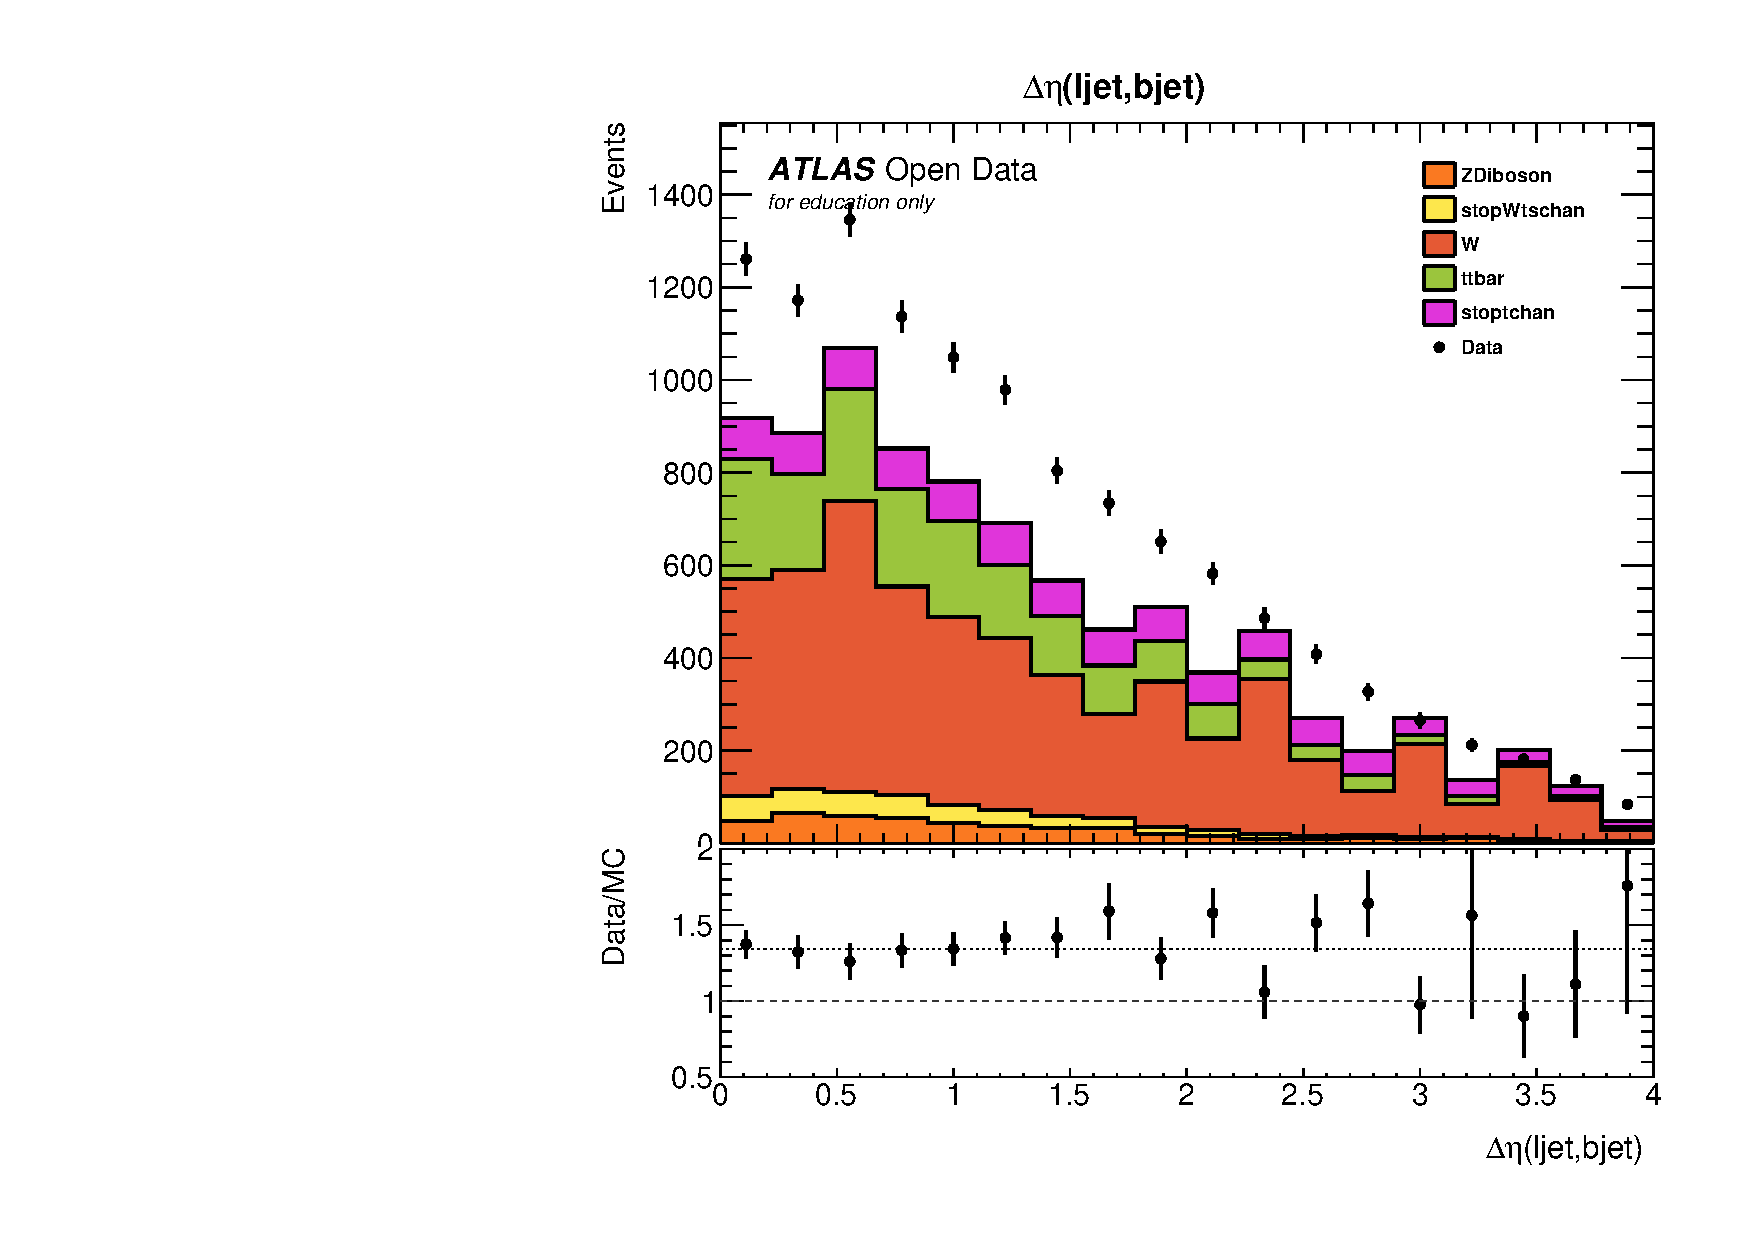
\includegraphics[scale=0.22]{dif} &
		
		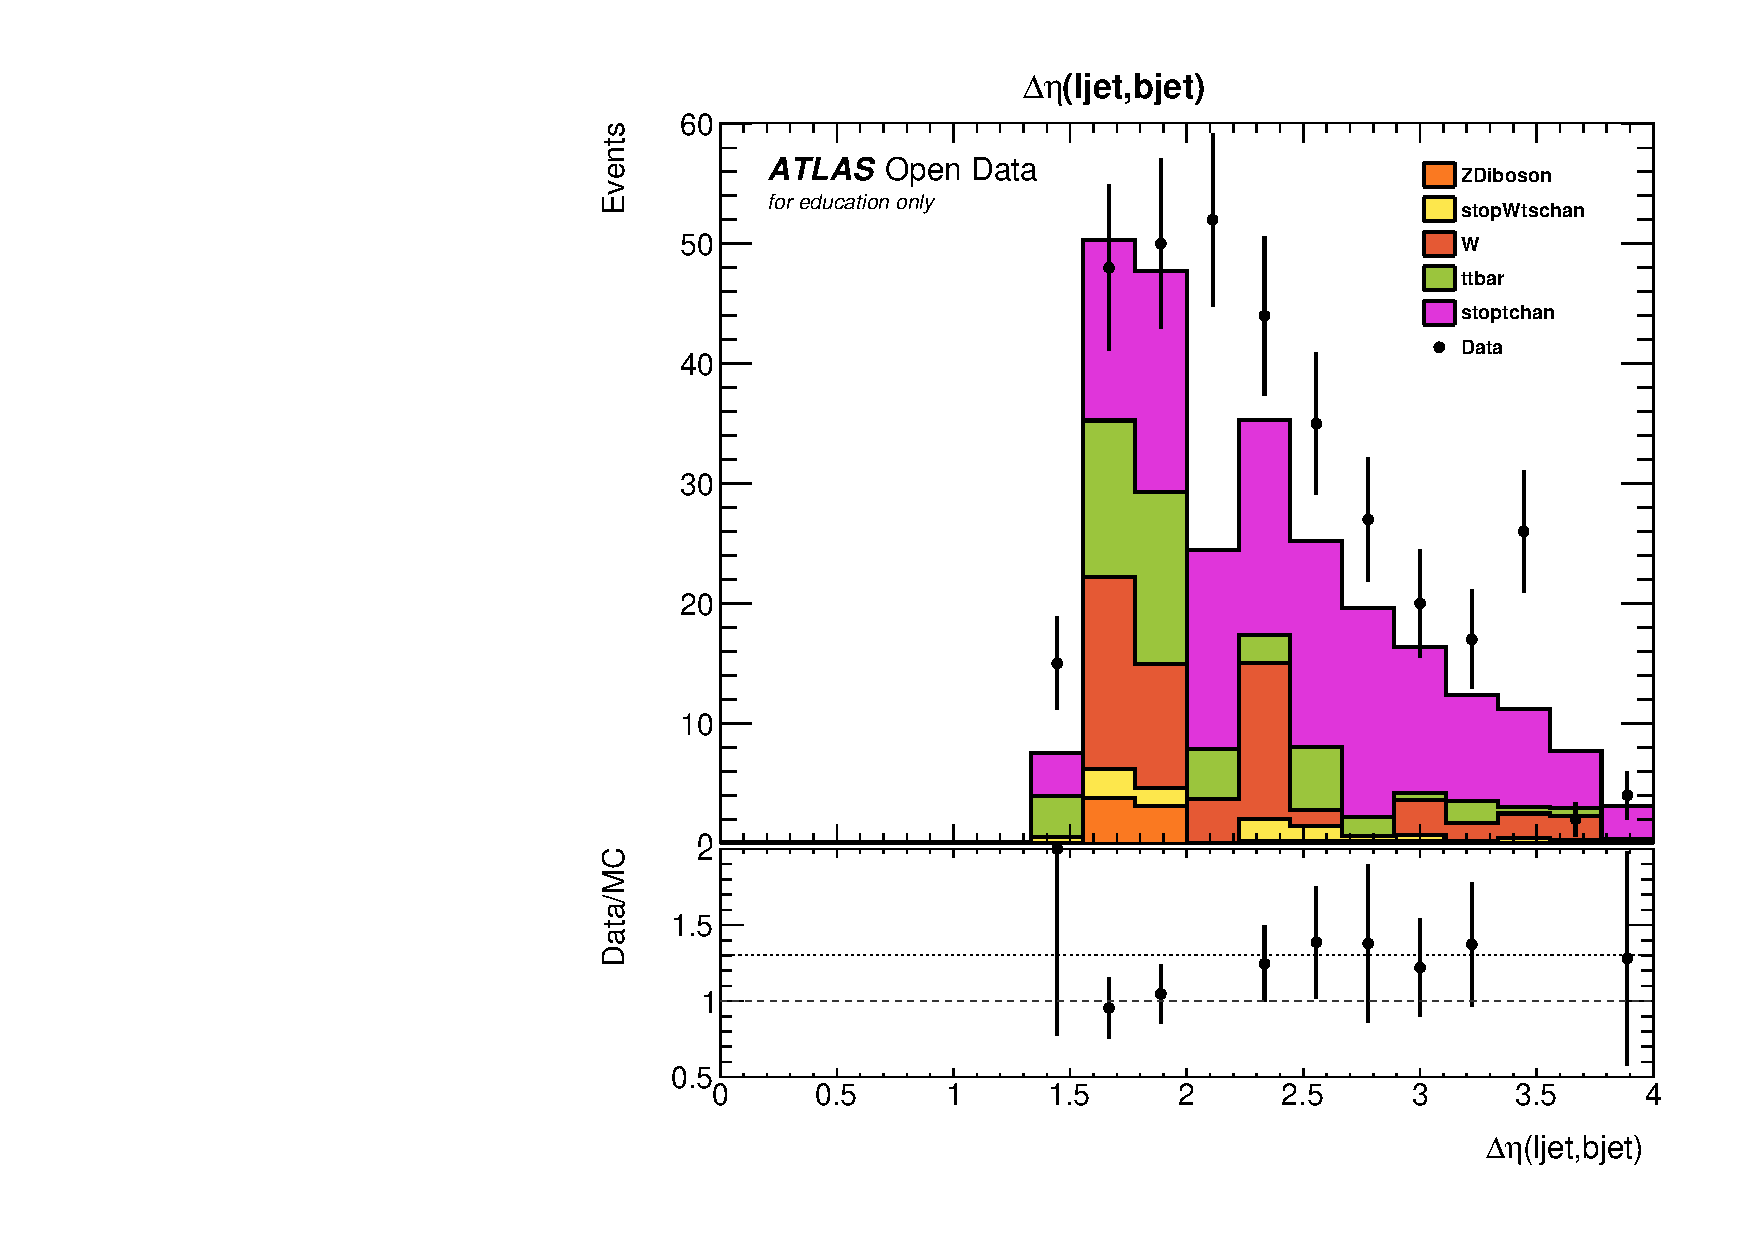
\includegraphics[scale=0.22]{dif_cuts} \\
		
		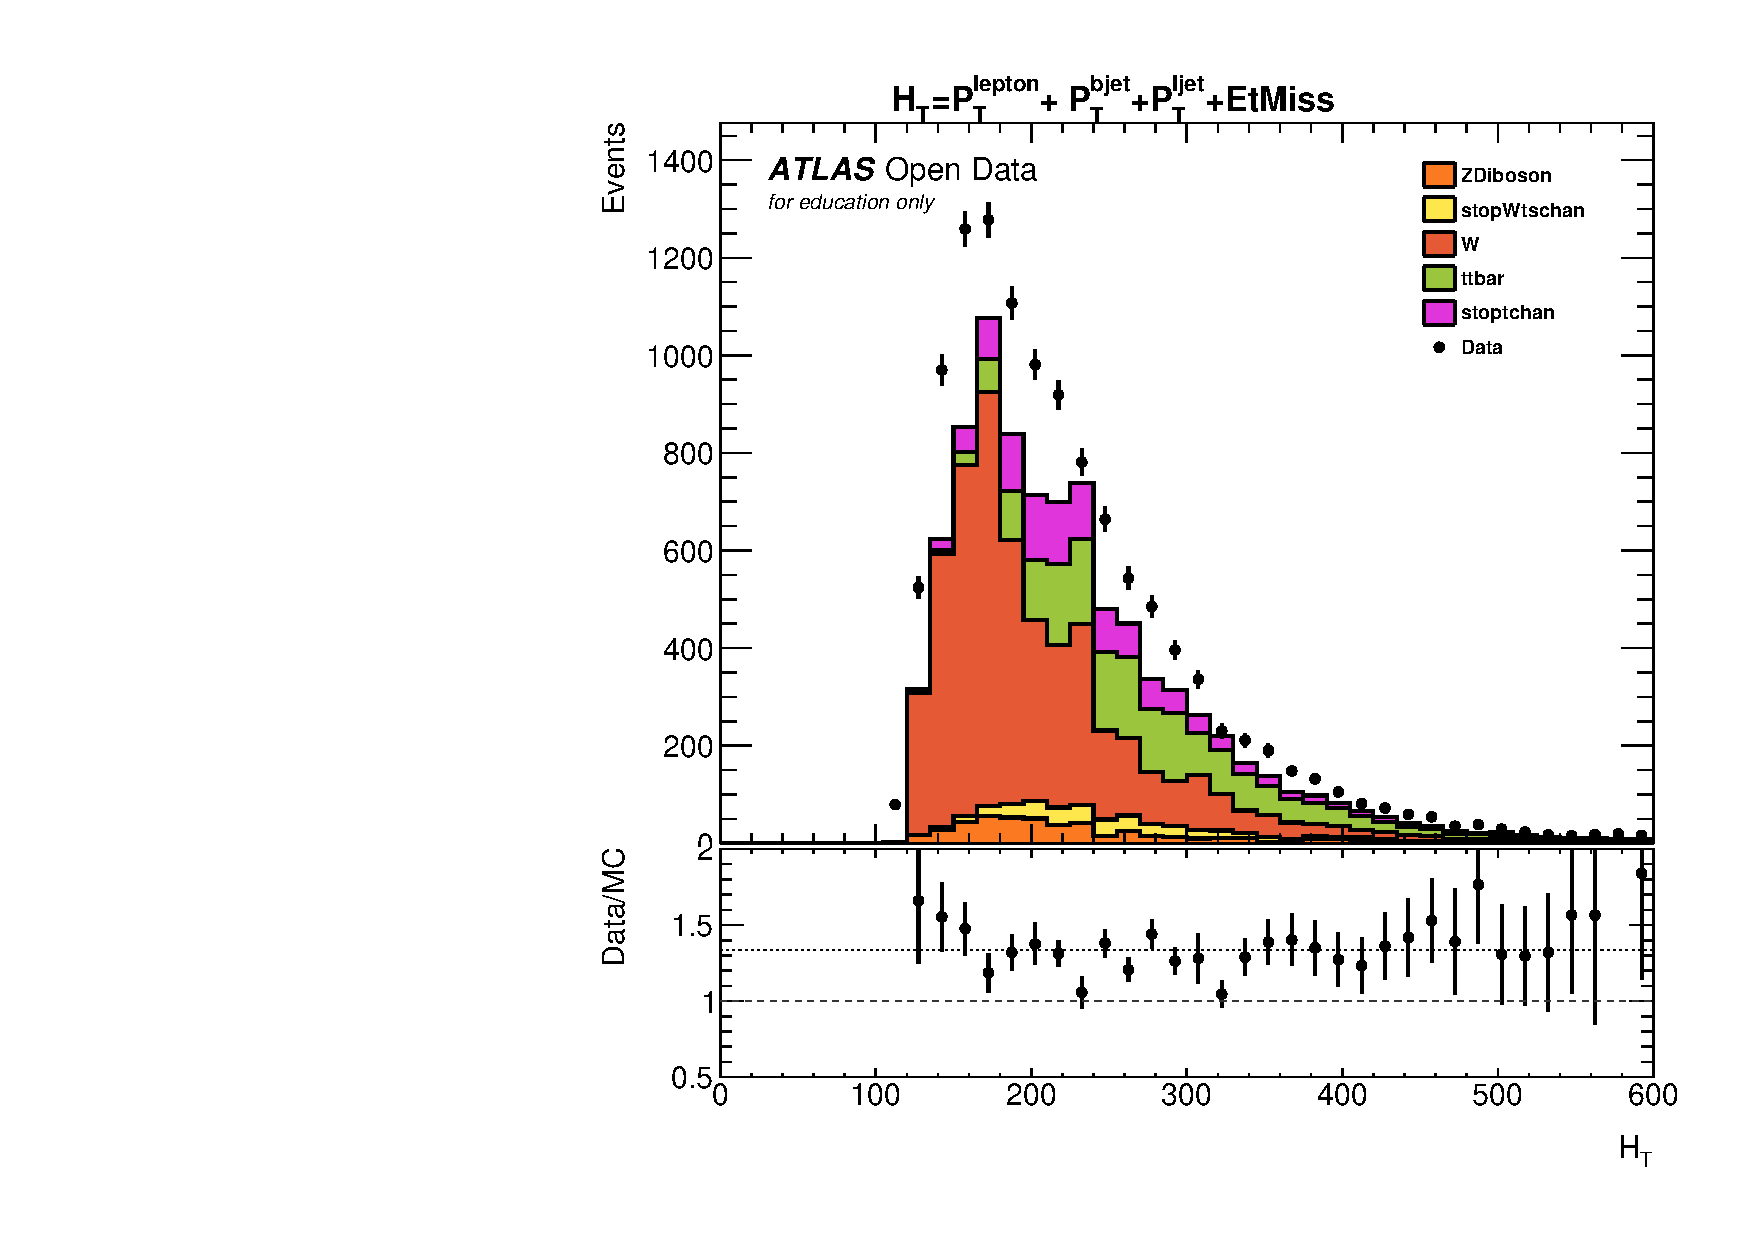
\includegraphics[scale=0.22]{Ht} &
		
		
		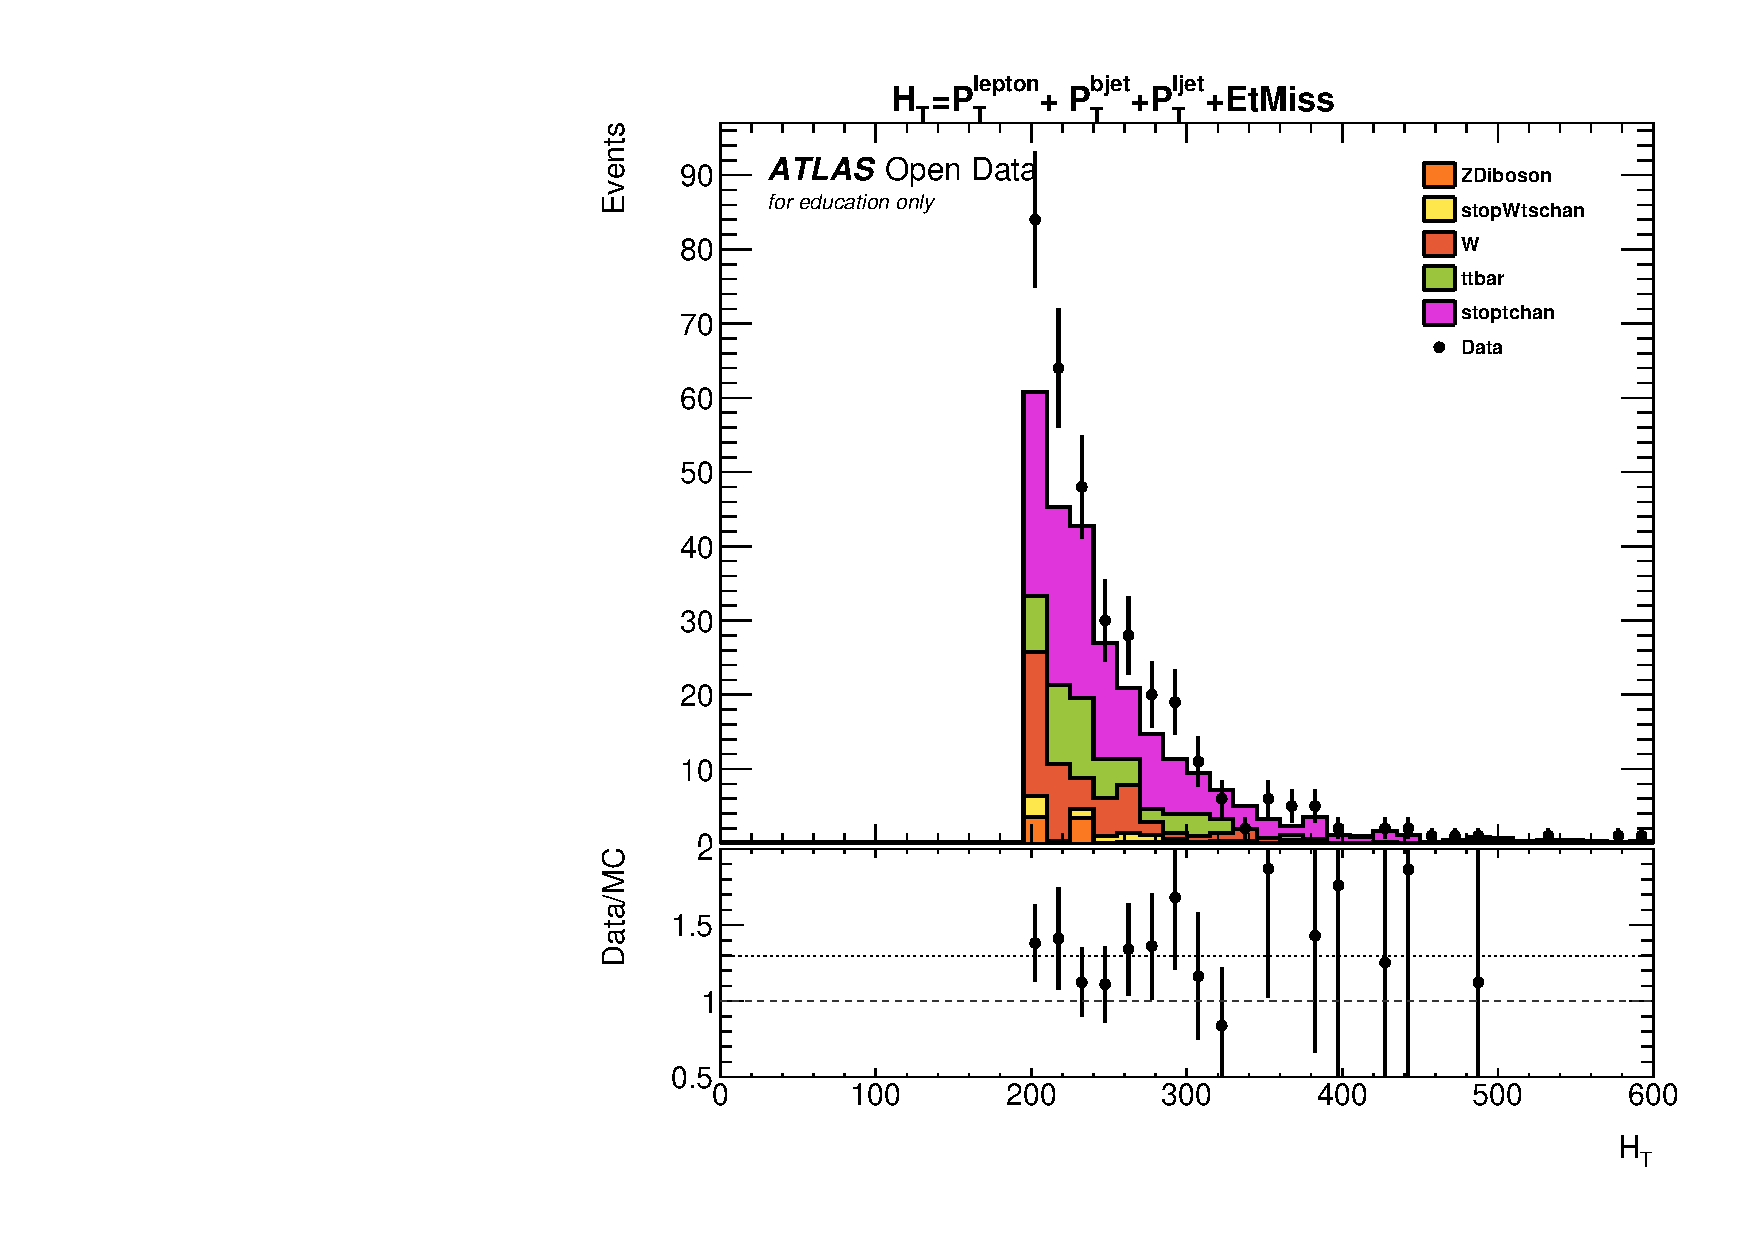
\includegraphics[scale=0.22]{Ht_cuts} 
		
		
		
	\end{tabular}
\end{center}
\end{frame}


\begin{frame}
	\begin{table}
		\centering
		\begin{tabular}{|c|c|c|}
			\hline
			\multicolumn{3}{|c|}{$N_{\text{evt}}$ ($\sqrt{s}=13$ TeV, $L_{\text{int}}=3.2$ fb$^{-1}$)} \\\hline
			Proceso & Preselección & Después de los cortes \\
			\hline\hline
			t-channel ($S$) & $1147\pm 13$& $153\pm5$ \\\hline
			 $t\bar{t}$ & $1853\pm41$& $64\pm7$\\
			  $W+$ jets &$5034\pm230$ & $80\pm 16$ \\
			   $Z$Diboson ($Z$+jets, $ZZ$, $ZW$, $WW$) & $478\pm 34$  & $4\pm 4$\\
			   	  stopWtchan (Wt,s-channel) & $395\pm5$ & $13\pm 1$\\\hline
			   	  	  Fondo total ($B$) &$7760$ & 160\\ \hline\hline
			   	  	  Datos reales &$11928$ & 396\\ \hline\hline
			   	  	  	  $\sigma=\tfrac{S}{\sqrt{S+B}}$ & 12.16 & 8.66 \\ \hline
			   	  	  	  	  $S/B$ & 0.15& 0.96\\
			    \hline
		\end{tabular}
	\end{table}
\end{frame}
\begin{frame}
\begin{center}
	\begin{tabular}{cc}
		
		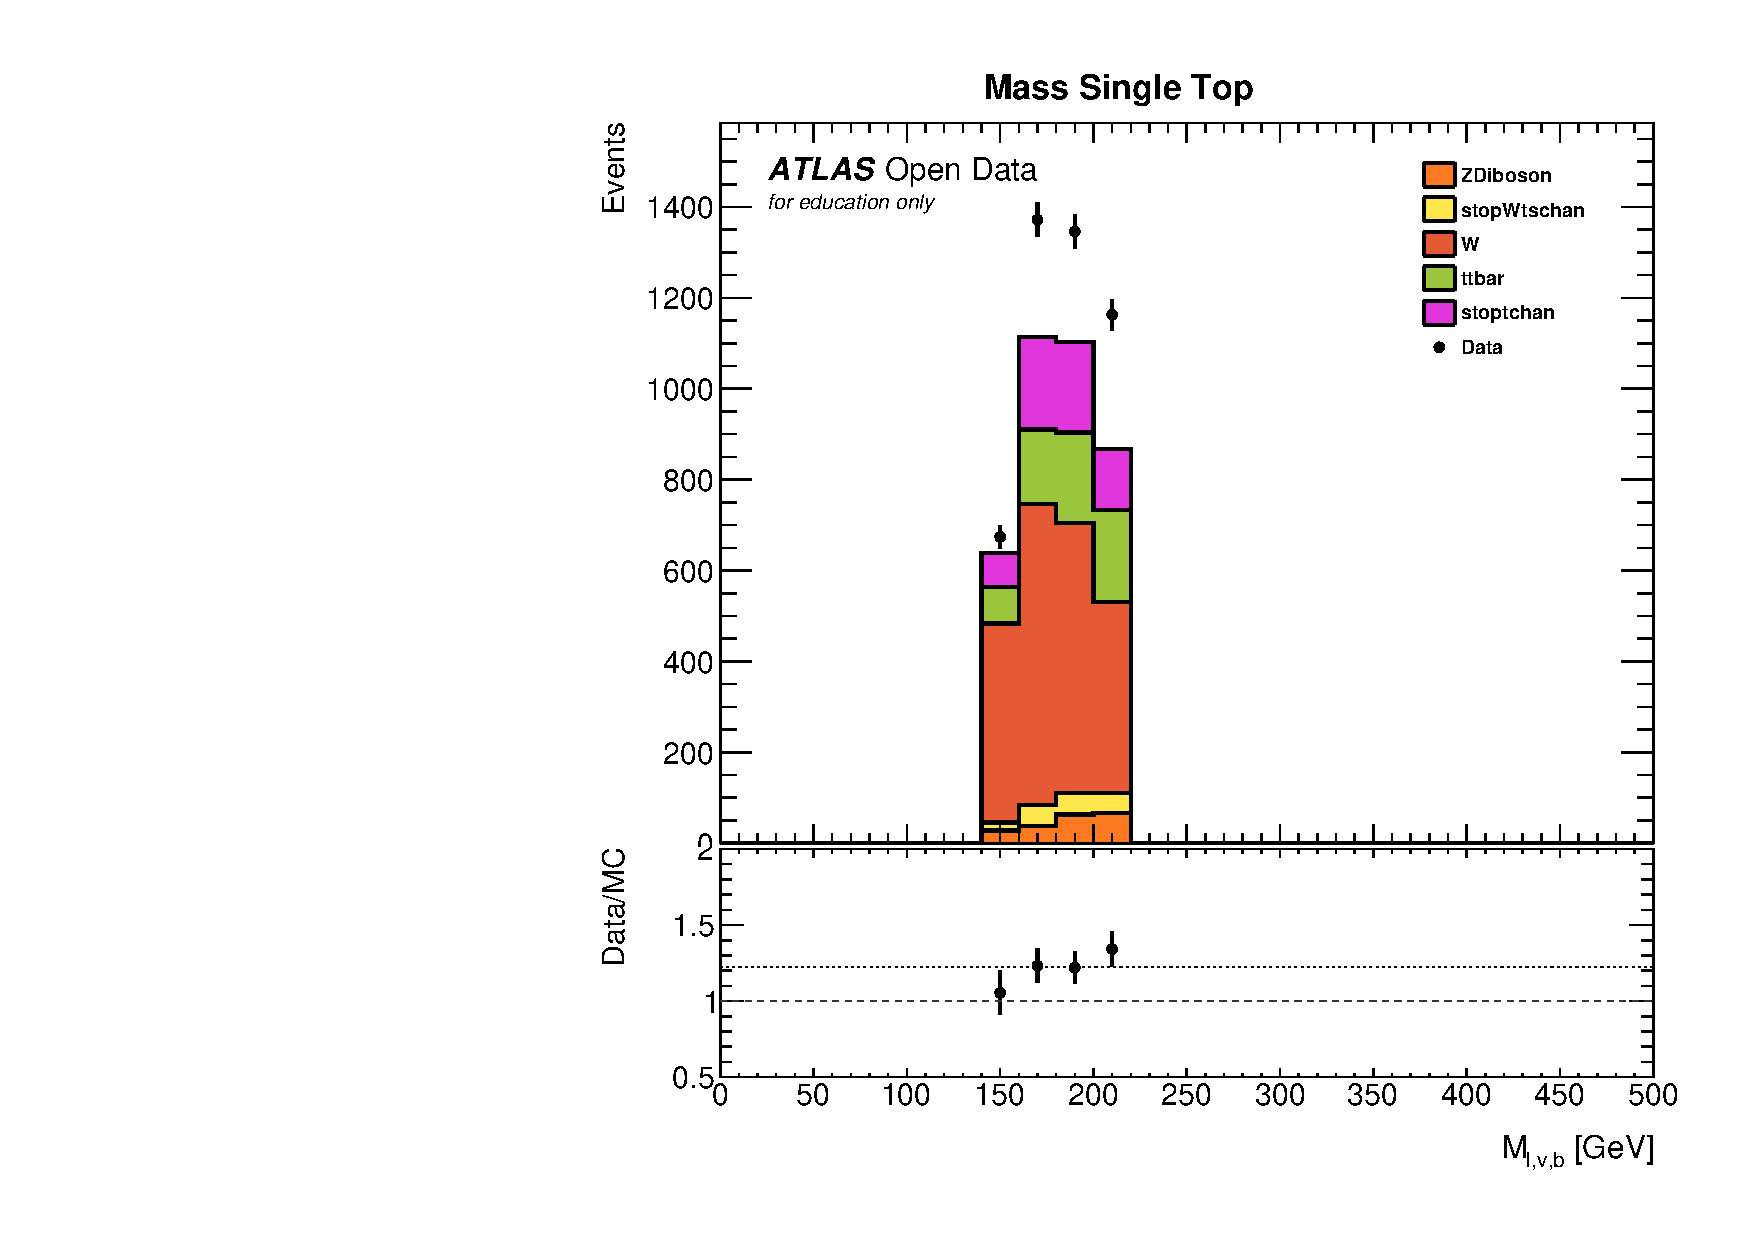
\includegraphics[scale=0.19]{SingleTopMasscarles} &
		
		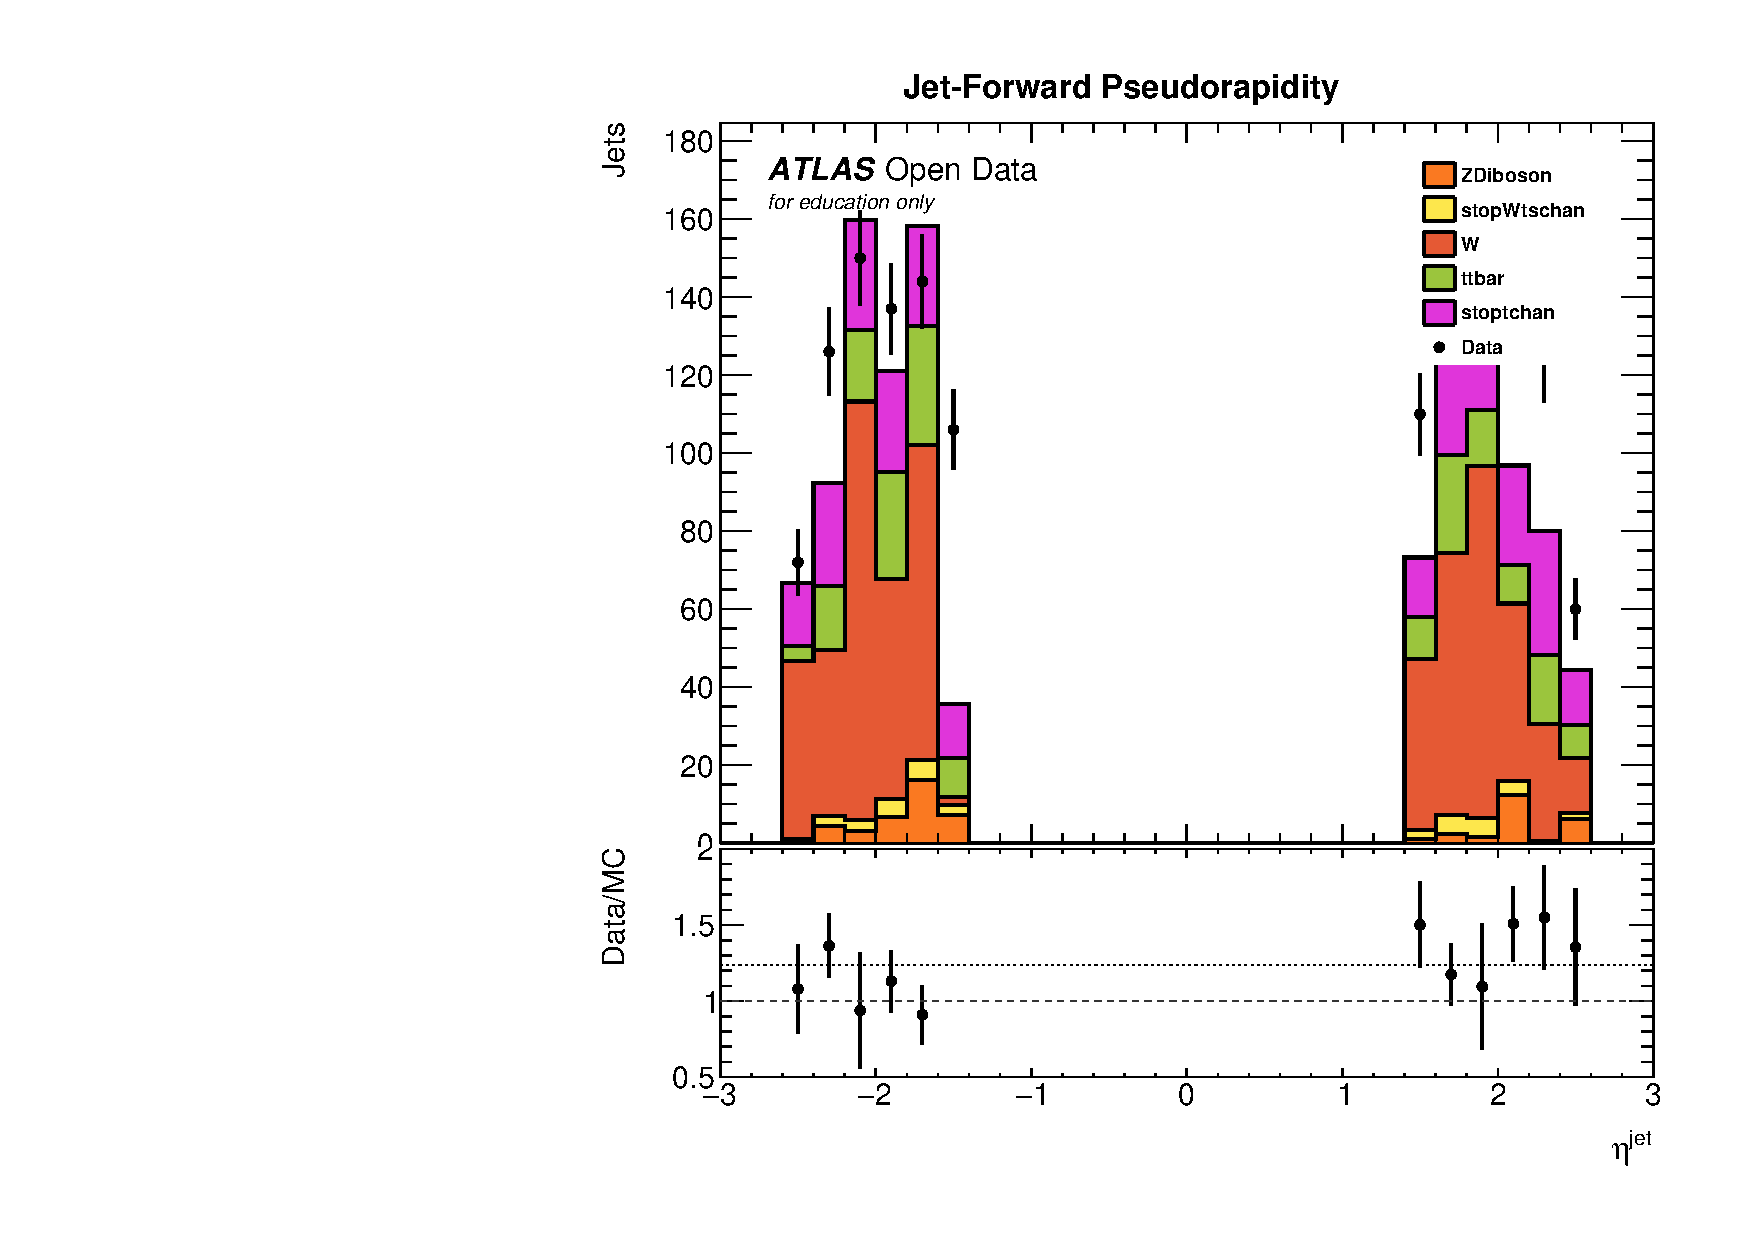
\includegraphics[scale=0.19]{jet_leta} \\
		$S/B=0.20$ $\sigma=10$ & $S/B=0.31$ $\sigma=8$ \\
		
		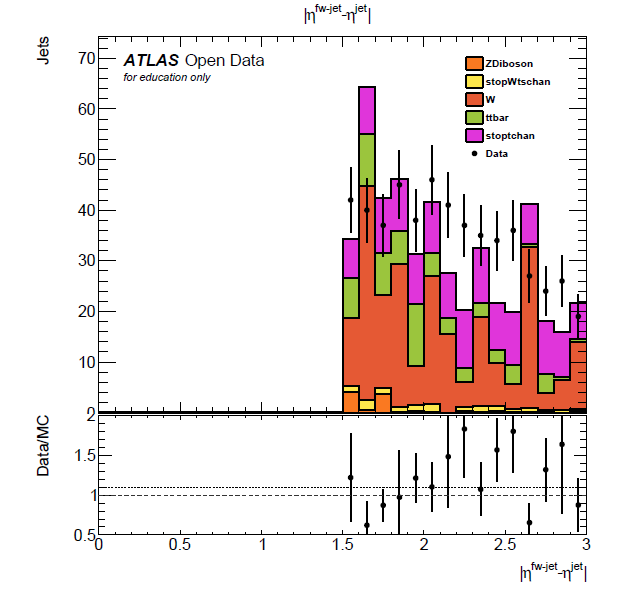
\includegraphics[scale=0.23]{deltaeta.png} &
		
		
		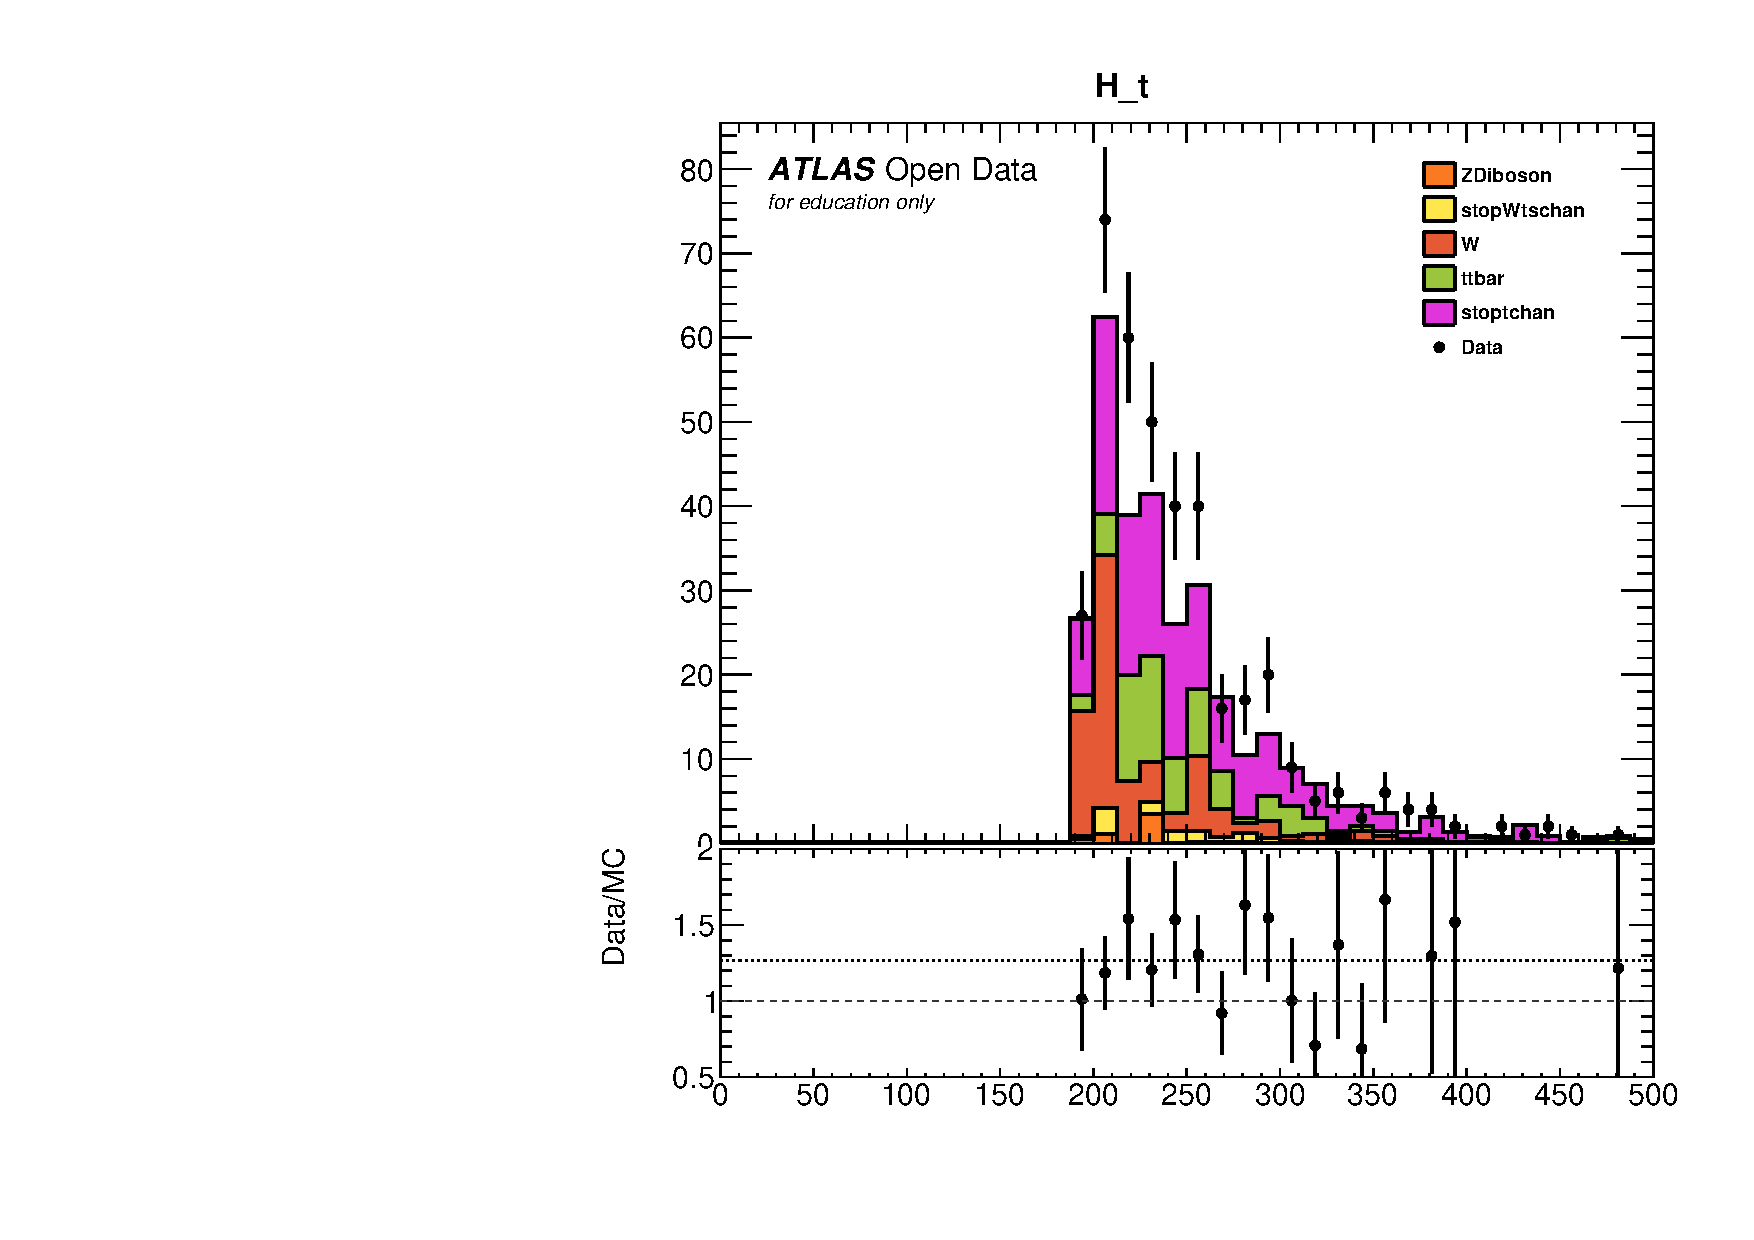
\includegraphics[scale=0.19]{htcarles} \\
			$S/B=0.55$ $\sigma=8$ & $S/B=0.96$ $\sigma=8.66$ 
		
		
	\end{tabular}
\end{center}
\end{frame}
\section{Estudio de la producción de un par top-antitop ($t\bar{t}$)}


\subsection{Estudio de reconstrucción de la masa y selección de señal}
\begin{frame}{Estudio de reconstrucción de la masa y selección de señal}
\begin{columns}
	\begin{column}{.5\textwidth}
	\color{blue}	Cortes previos (preselección):
		\begin{itemize}
			\item Procesos con al menos $4$ jets: 2 procedentes de uno de los $W$ y 2 b-jets
			\item Un leptón cargado ($e$ o $\mu$) y aislado. Procedente del $W$
			\item $E_T^{\text{miss}}>30$ GeV vinculada a los neutrinos
		\end{itemize}
		\end{column}
	\begin{column}{.32\textwidth}
		\begin{figure}
	\centering
	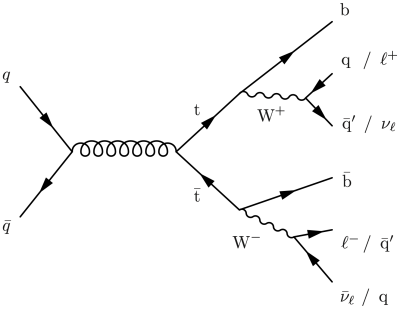
\includegraphics[scale=0.3]{ttbar.png}

\end{figure}
\end{column}
\end{columns}
Buscamos 3 jets que maximicen $(\sum_{i=1}^3p_i).Pt()\rightarrow$ $M_{\text{top}}$

Entre los anteriores se buscan 2 jets que maximicen $(\sum_{i=1}^2 p_i).Pt()\rightarrow M_{W}$

\color{blue}Corte de selección:
\begin{itemize}
	\item $70$ GeV $<$ $M_{\text{rec}}^W$ $<$ 90 GeV
\end{itemize}
\end{frame}

\begin{frame}
\begin{center}
	\begin{tabular}{cc}
		
			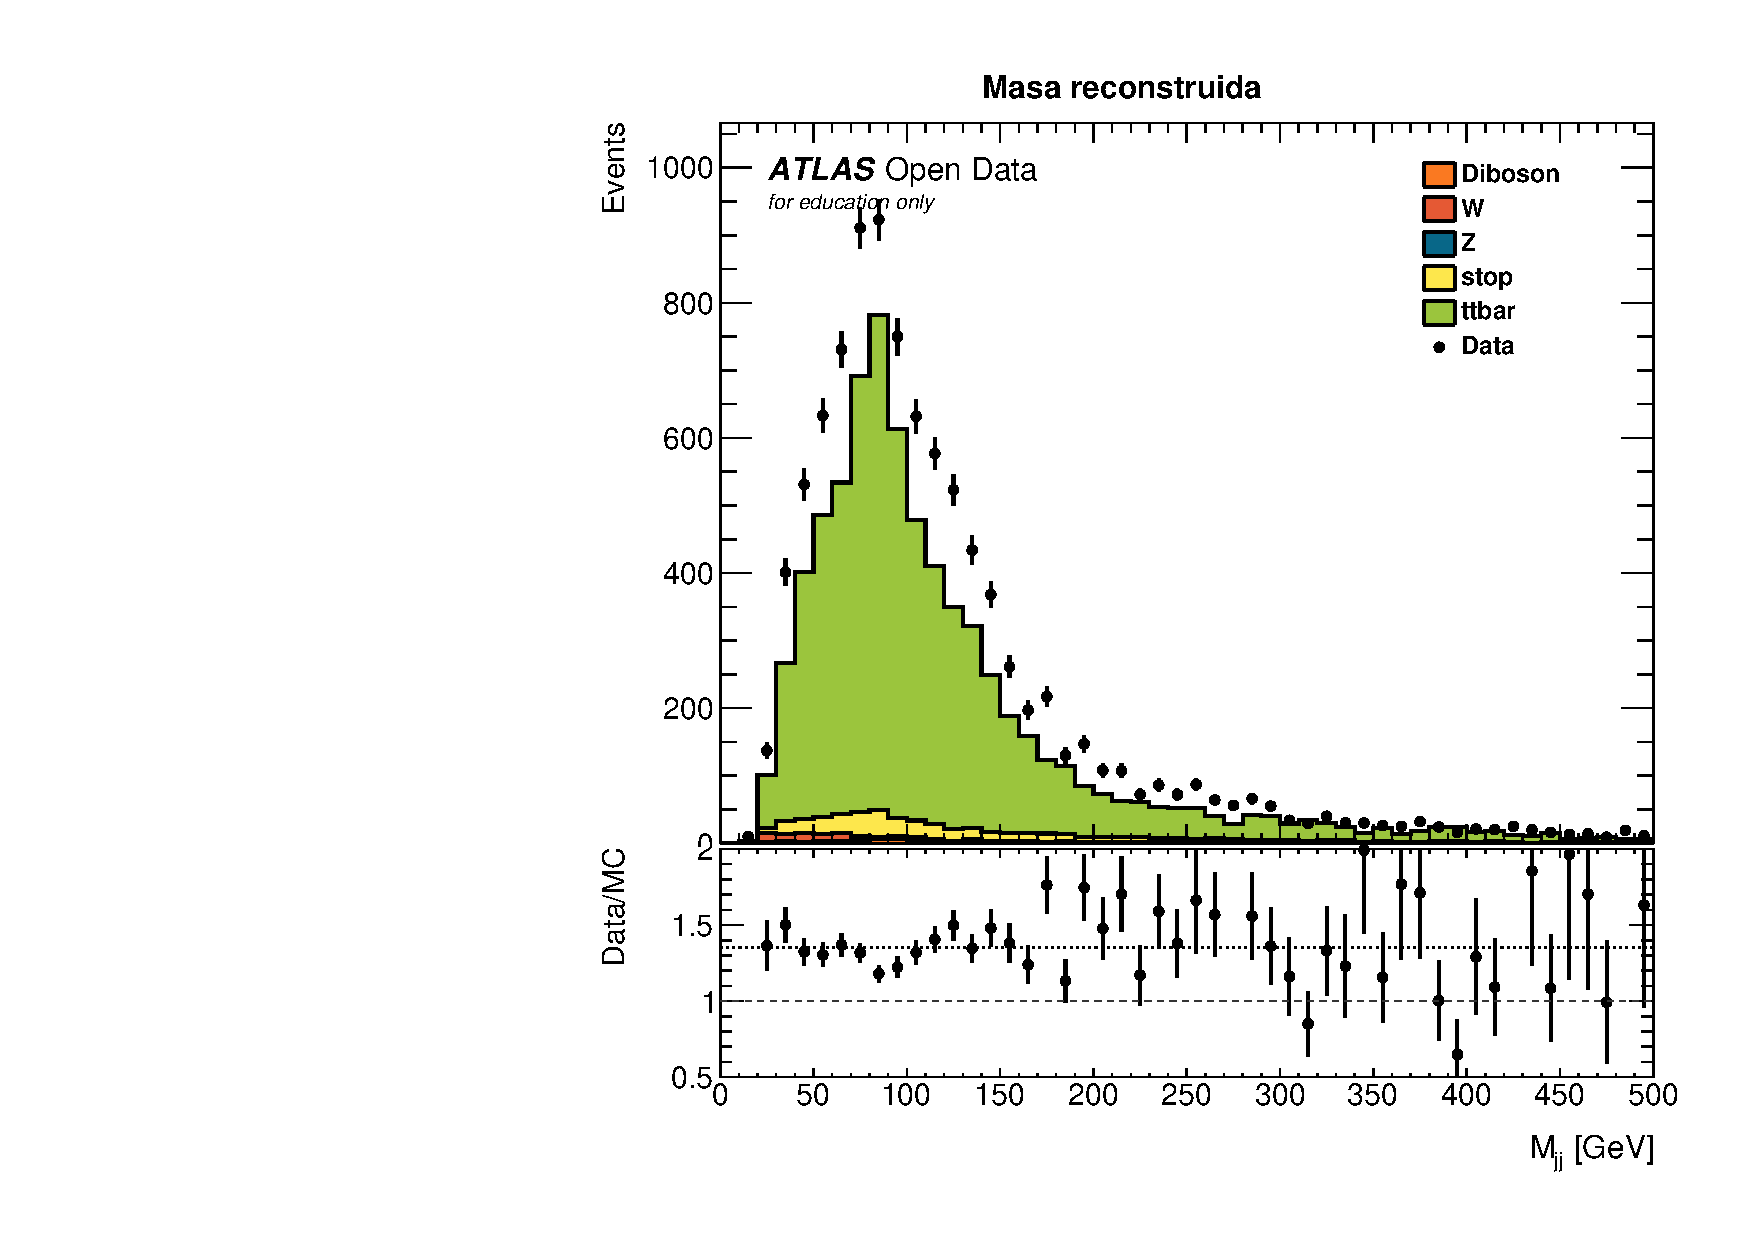
\includegraphics[scale=0.22]{recoWmass} &
		
		
		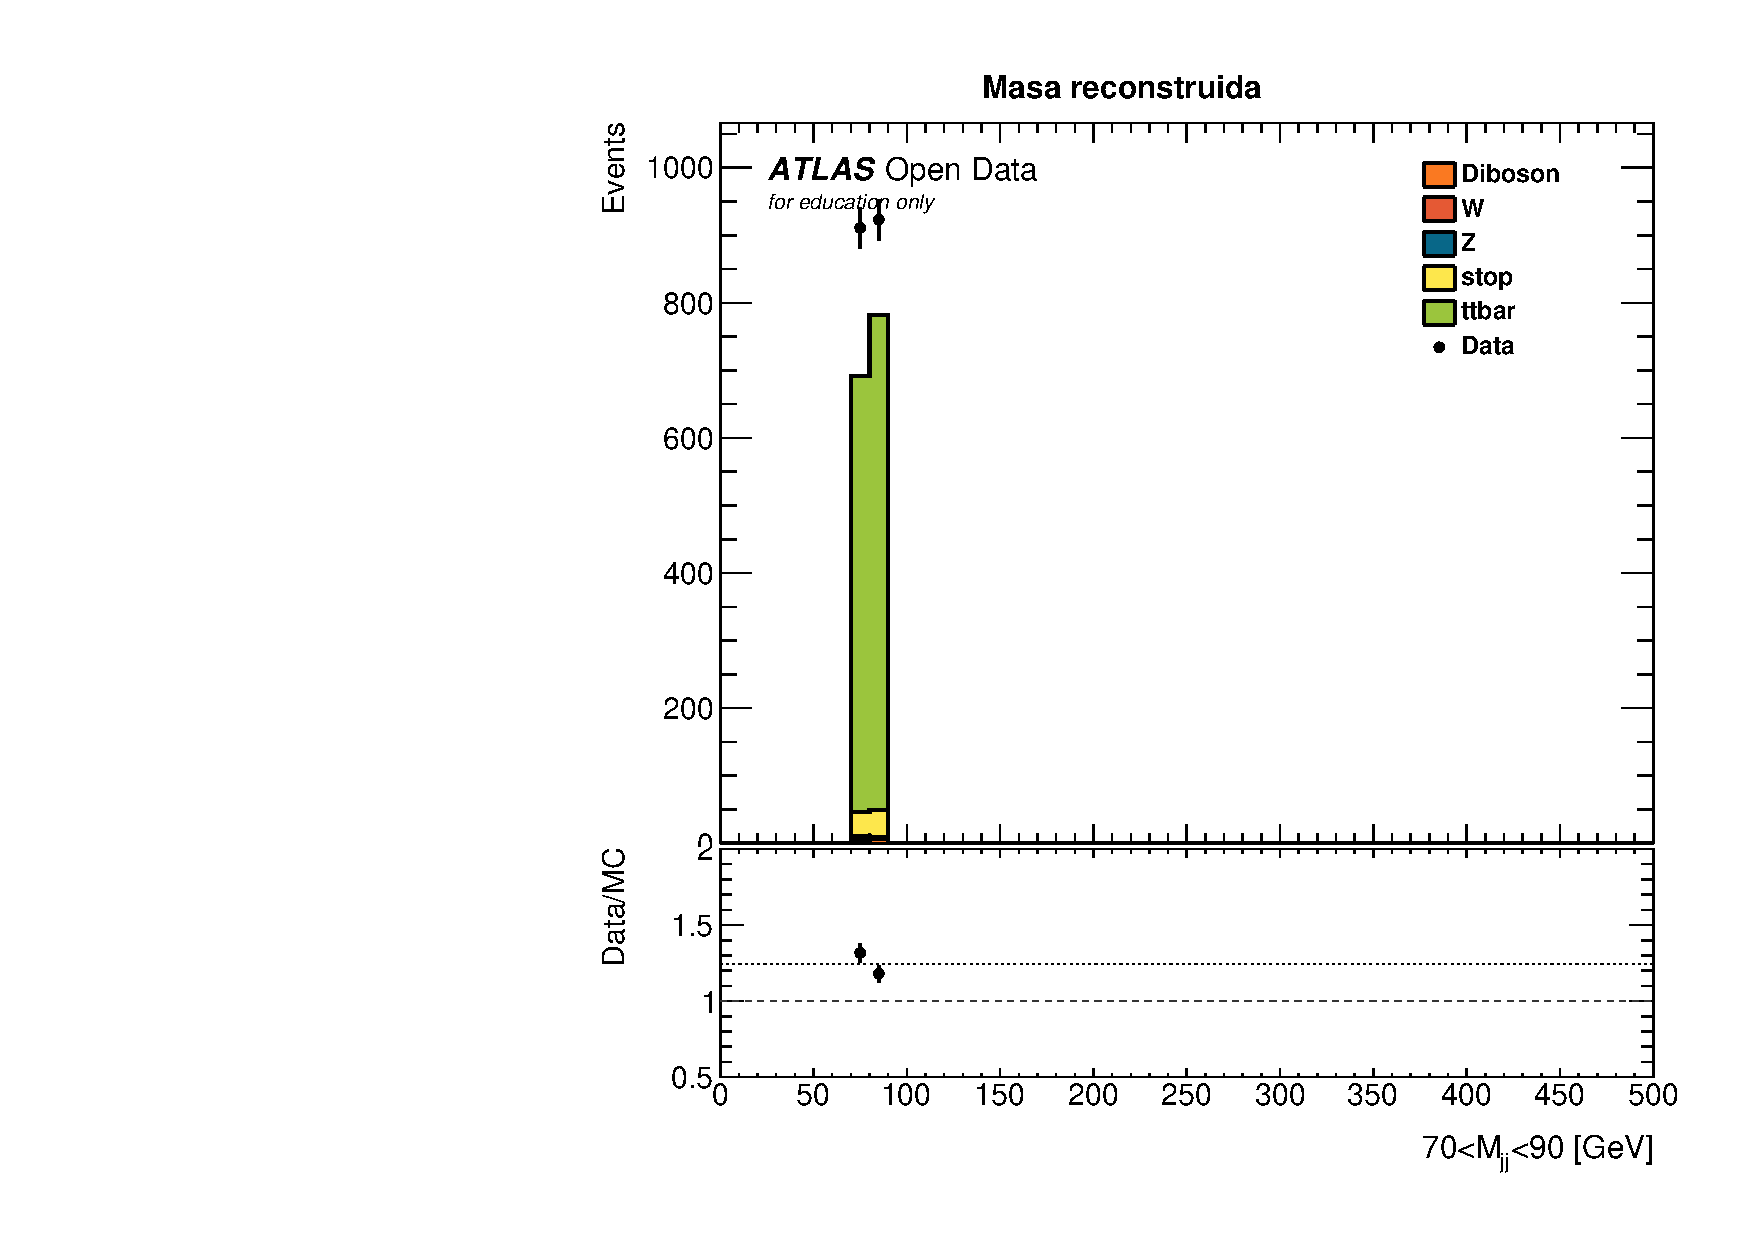
\includegraphics[scale=0.22]{recoWmassbis} \\
		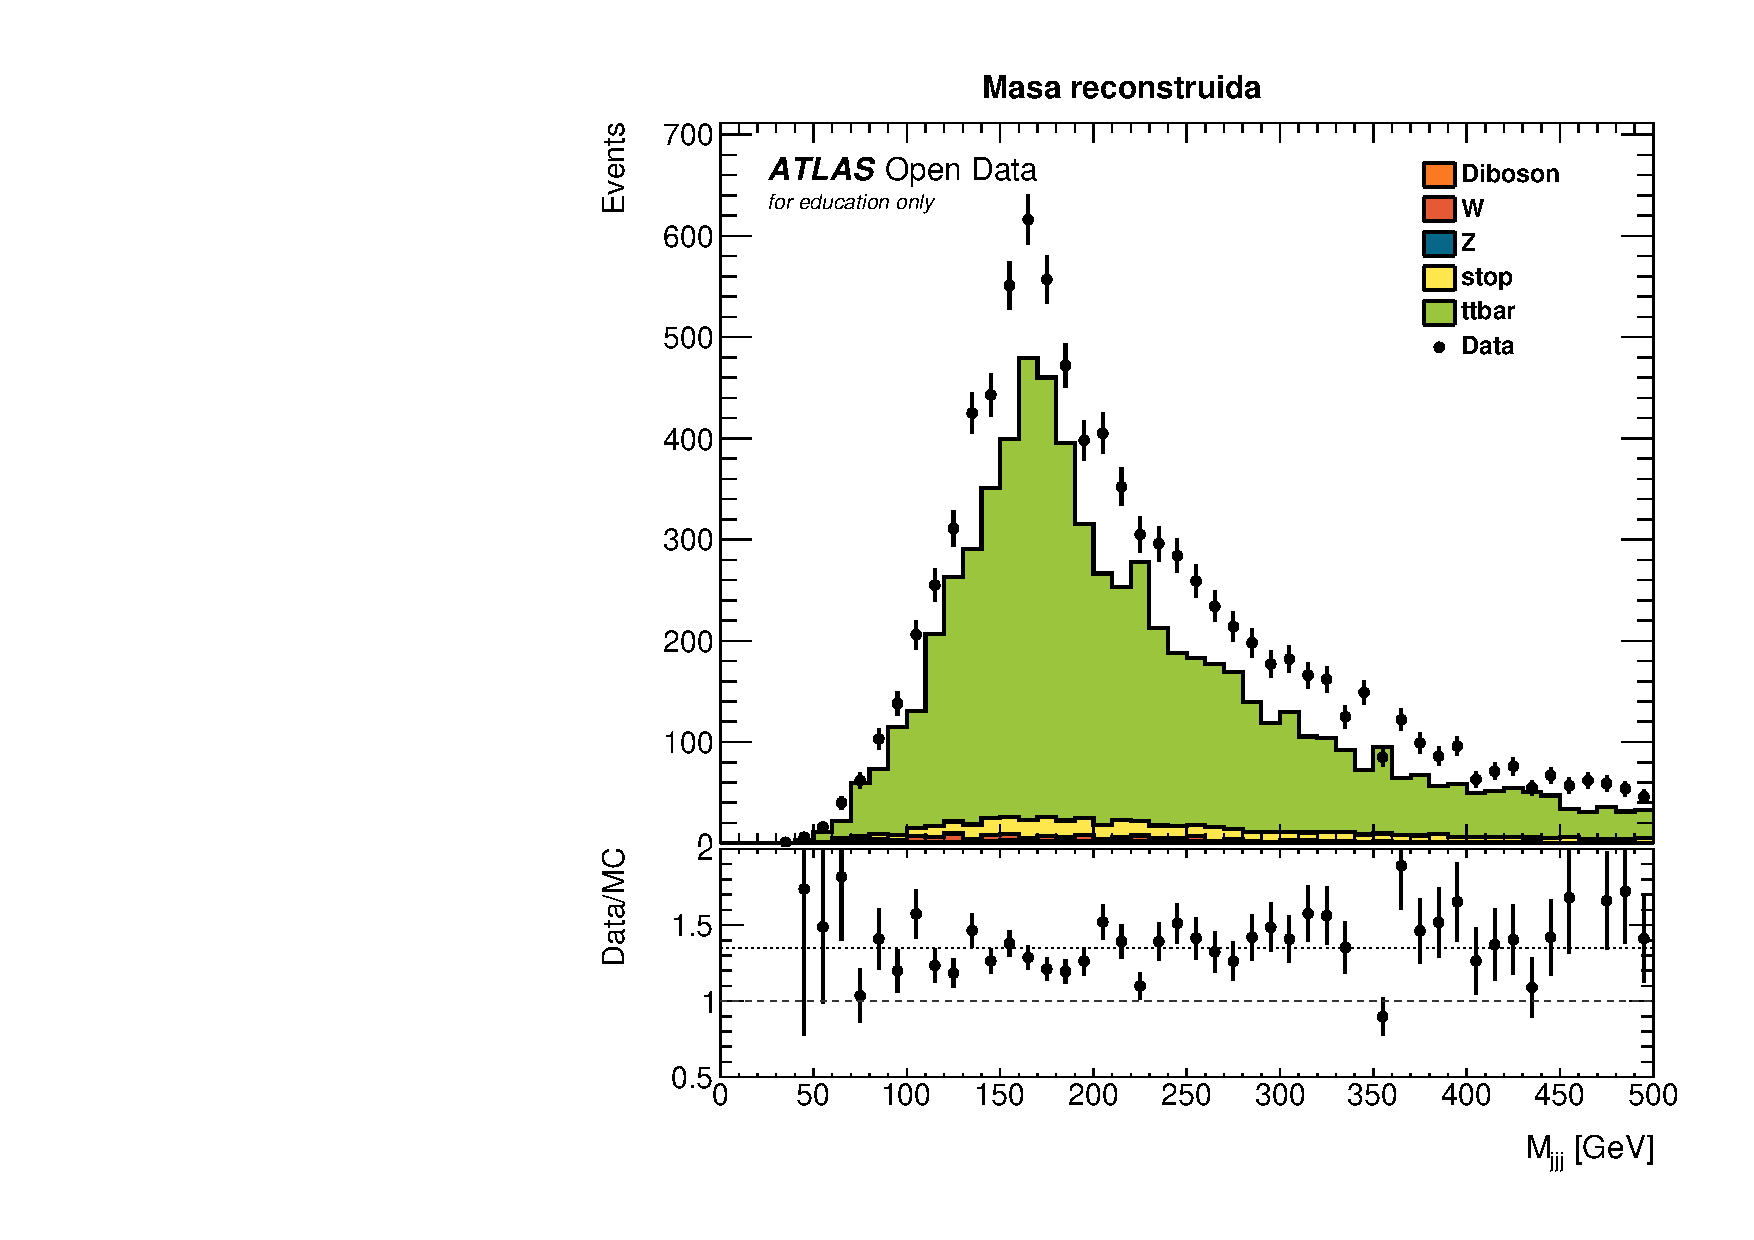
\includegraphics[scale=0.22]{reconsmass} &
		
		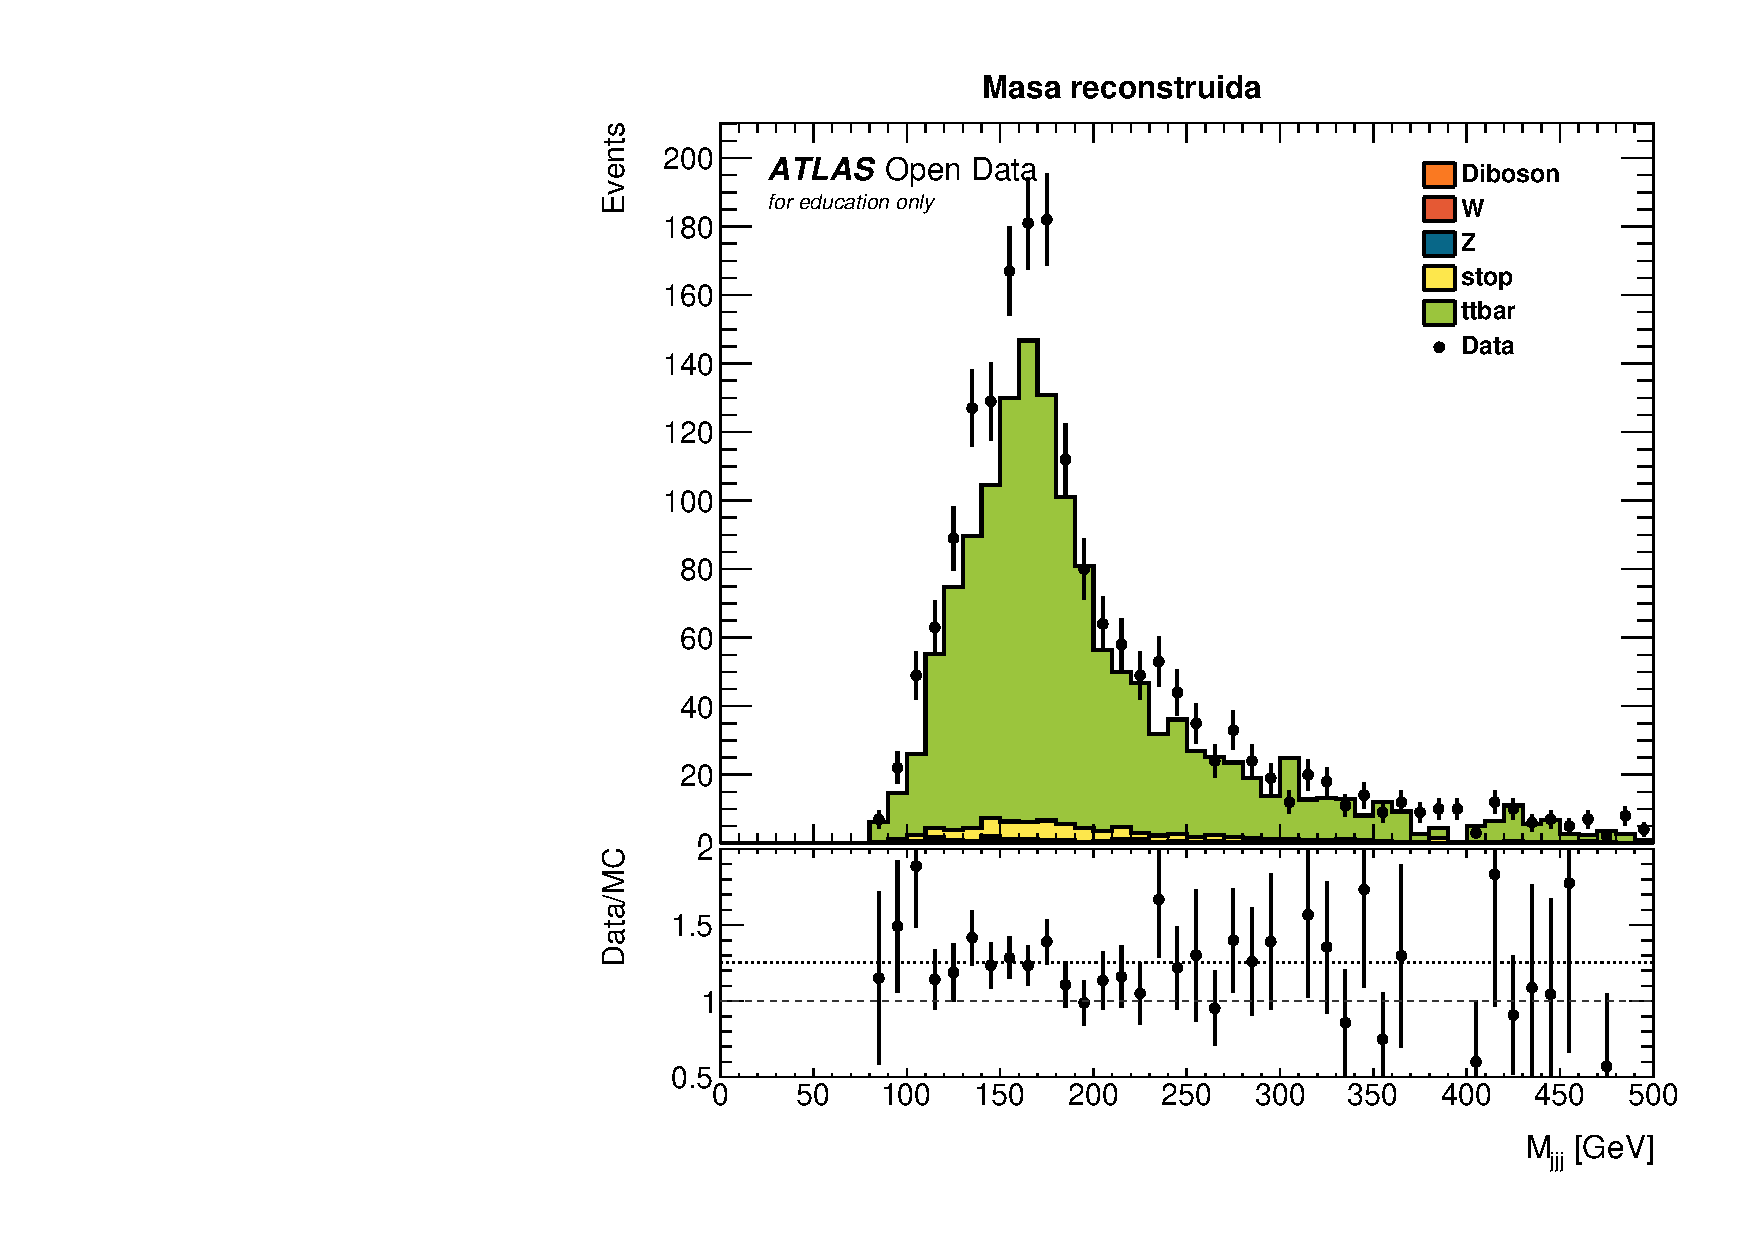
\includegraphics[scale=0.22]{reconsmassbis} \\
		
	

		
	\end{tabular}
\end{center}
\end{frame}
\section{Conclusiones}
\begin{frame}{Conclusiones}
\begin{itemize}
	\item Se ha contribuido a la validación y puesta a punto del nuevo ATLAS Open Data a $\sqrt{s}=13$ TeV con análisis de física del top.
	\item Producción de un solo top en el canal t:\begin{itemize}
	\item Análisis de generador.
	\item Ejercicio de reconstrucción de la masa y determinación del $p_z$ del neutrino.
	
	\item Selección de una muestra enriquecida en señal basada en cortes secuenciales (cuantificación del cociente $S/B$ i de $\sigma$). \end{itemize}
	\item Producción $t\bar{t}$:
	\begin{itemize}
		\item Se ha realizado un análisis de la selección y un estudio de la reconstrucción de la masa.
	\end{itemize}
\item Se ha contribuido de las infraestructuras de análisis tanto en C++ como en Python del nuevo ATLAS Open Data.
\item Desde el punto de vista de la física del top tanto las muestras simuladas como de datos reales y la infraestructura de análisis parecen adecuadas para estudiantes.
\end{itemize}
\end{frame}
\begin{frame}{Agradecimientos}
\begin{itemize}
\item	Agradacemos al IFIC la oportunidad de participar en esta escuela de verano, al grupo ATLAS por su acogida, a todos los tutores y especialmente a Susana Cabrera.
\item Agradecemos al grupo de la colaboración ATLAS por permitirnos utilizar las muestras y la infraestructura de análisis del nuevo ATLAS Open Data a $\sqrt{s}=13$ TeV.
\end{itemize}
\end{frame}

\end{document}

